% Options for packages loaded elsewhere
% Options for packages loaded elsewhere
\PassOptionsToPackage{unicode}{hyperref}
\PassOptionsToPackage{hyphens}{url}
\PassOptionsToPackage{dvipsnames,svgnames,x11names}{xcolor}
%
\documentclass[
  10pt,
  letterpaper,
  DIV=11,
  numbers=noendperiod]{scrartcl}
\usepackage{xcolor}
\usepackage[a4paper,top=2cm,bottom=2.5cm,left=2cm,right=2cm,heightrounded,footskip=1cm]{geometry}
\usepackage{amsmath,amssymb}
\setcounter{secnumdepth}{4}
\usepackage{iftex}
\ifPDFTeX
  \usepackage[T1]{fontenc}
  \usepackage[utf8]{inputenc}
  \usepackage{textcomp} % provide euro and other symbols
\else % if luatex or xetex
  \usepackage{unicode-math} % this also loads fontspec
  \defaultfontfeatures{Scale=MatchLowercase}
  \defaultfontfeatures[\rmfamily]{Ligatures=TeX,Scale=1}
\fi
\usepackage{lmodern}
\ifPDFTeX\else
  % xetex/luatex font selection
  \setmainfont[]{Latin Modern Roman}
  \setsansfont[]{Latin Modern Roman}
\fi
% Use upquote if available, for straight quotes in verbatim environments
\IfFileExists{upquote.sty}{\usepackage{upquote}}{}
\IfFileExists{microtype.sty}{% use microtype if available
  \usepackage[]{microtype}
  \UseMicrotypeSet[protrusion]{basicmath} % disable protrusion for tt fonts
}{}
\usepackage{setspace}
\makeatletter
\@ifundefined{KOMAClassName}{% if non-KOMA class
  \IfFileExists{parskip.sty}{%
    \usepackage{parskip}
  }{% else
    \setlength{\parindent}{0pt}
    \setlength{\parskip}{6pt plus 2pt minus 1pt}}
}{% if KOMA class
  \KOMAoptions{parskip=half}}
\makeatother
% Make \paragraph and \subparagraph free-standing
\makeatletter
\ifx\paragraph\undefined\else
  \let\oldparagraph\paragraph
  \renewcommand{\paragraph}{
    \@ifstar
      \xxxParagraphStar
      \xxxParagraphNoStar
  }
  \newcommand{\xxxParagraphStar}[1]{\oldparagraph*{#1}\mbox{}}
  \newcommand{\xxxParagraphNoStar}[1]{\oldparagraph{#1}\mbox{}}
\fi
\ifx\subparagraph\undefined\else
  \let\oldsubparagraph\subparagraph
  \renewcommand{\subparagraph}{
    \@ifstar
      \xxxSubParagraphStar
      \xxxSubParagraphNoStar
  }
  \newcommand{\xxxSubParagraphStar}[1]{\oldsubparagraph*{#1}\mbox{}}
  \newcommand{\xxxSubParagraphNoStar}[1]{\oldsubparagraph{#1}\mbox{}}
\fi
\makeatother


\usepackage{longtable,booktabs,array}
\usepackage{calc} % for calculating minipage widths
% Correct order of tables after \paragraph or \subparagraph
\usepackage{etoolbox}
\makeatletter
\patchcmd\longtable{\par}{\if@noskipsec\mbox{}\fi\par}{}{}
\makeatother
% Allow footnotes in longtable head/foot
\IfFileExists{footnotehyper.sty}{\usepackage{footnotehyper}}{\usepackage{footnote}}
\makesavenoteenv{longtable}
\usepackage{graphicx}
\makeatletter
\newsavebox\pandoc@box
\newcommand*\pandocbounded[1]{% scales image to fit in text height/width
  \sbox\pandoc@box{#1}%
  \Gscale@div\@tempa{\textheight}{\dimexpr\ht\pandoc@box+\dp\pandoc@box\relax}%
  \Gscale@div\@tempb{\linewidth}{\wd\pandoc@box}%
  \ifdim\@tempb\p@<\@tempa\p@\let\@tempa\@tempb\fi% select the smaller of both
  \ifdim\@tempa\p@<\p@\scalebox{\@tempa}{\usebox\pandoc@box}%
  \else\usebox{\pandoc@box}%
  \fi%
}
% Set default figure placement to htbp
\def\fps@figure{htbp}
\makeatother


% definitions for citeproc citations
\NewDocumentCommand\citeproctext{}{}
\NewDocumentCommand\citeproc{mm}{%
  \begingroup\def\citeproctext{#2}\cite{#1}\endgroup}
\makeatletter
 % allow citations to break across lines
 \let\@cite@ofmt\@firstofone
 % avoid brackets around text for \cite:
 \def\@biblabel#1{}
 \def\@cite#1#2{{#1\if@tempswa , #2\fi}}
\makeatother
\newlength{\cslhangindent}
\setlength{\cslhangindent}{1.5em}
\newlength{\csllabelwidth}
\setlength{\csllabelwidth}{3em}
\newenvironment{CSLReferences}[2] % #1 hanging-indent, #2 entry-spacing
 {\begin{list}{}{%
  \setlength{\itemindent}{0pt}
  \setlength{\leftmargin}{0pt}
  \setlength{\parsep}{0pt}
  % turn on hanging indent if param 1 is 1
  \ifodd #1
   \setlength{\leftmargin}{\cslhangindent}
   \setlength{\itemindent}{-1\cslhangindent}
  \fi
  % set entry spacing
  \setlength{\itemsep}{#2\baselineskip}}}
 {\end{list}}
\usepackage{calc}
\newcommand{\CSLBlock}[1]{\hfill\break\parbox[t]{\linewidth}{\strut\ignorespaces#1\strut}}
\newcommand{\CSLLeftMargin}[1]{\parbox[t]{\csllabelwidth}{\strut#1\strut}}
\newcommand{\CSLRightInline}[1]{\parbox[t]{\linewidth - \csllabelwidth}{\strut#1\strut}}
\newcommand{\CSLIndent}[1]{\hspace{\cslhangindent}#1}



\setlength{\emergencystretch}{3em} % prevent overfull lines

\providecommand{\tightlist}{%
  \setlength{\itemsep}{0pt}\setlength{\parskip}{0pt}}



 


\usepackage{booktabs}
\usepackage{longtable}
\usepackage{array}
\usepackage{multirow}
\usepackage{wrapfig}
\usepackage{float}
\usepackage{colortbl}
\usepackage{pdflscape}
\usepackage{tabu}
\usepackage{threeparttable}
\usepackage{threeparttablex}
\usepackage[normalem]{ulem}
\usepackage{makecell}
\usepackage{xcolor}
\usepackage{setspace}
\usepackage{tikz}
\usetikzlibrary{arrows.meta, positioning, fit}
\linespread{1.2}
\usepackage{changepage}
\usepackage{longtable}
\usepackage{nameref}
\usepackage{hyperref}
\usepackage{booktabs}
\usepackage{tabularray}
\usepackage{float}
\usepackage{etoolbox}
\makeatletter



\renewcommand\section{\@startsection{section}{1}{\z@}%
  {-3.5ex \@plus -1ex \@minus -.2ex}%
  {2.3ex \@plus.2ex}%
  {\normalfont\Large\bfseries\centering}}
\counterwithin{figure}{section}
\counterwithin{table}{section}
\makeatother
\KOMAoption{captions}{tableheading}
\makeatletter
\@ifpackageloaded{caption}{}{\usepackage{caption}}
\AtBeginDocument{%
\ifdefined\contentsname
  \renewcommand*\contentsname{Table of contents}
\else
  \newcommand\contentsname{Table of contents}
\fi
\ifdefined\listfigurename
  \renewcommand*\listfigurename{List of Figures}
\else
  \newcommand\listfigurename{List of Figures}
\fi
\ifdefined\listtablename
  \renewcommand*\listtablename{List of Tables}
\else
  \newcommand\listtablename{List of Tables}
\fi
\ifdefined\figurename
  \renewcommand*\figurename{Figure}
\else
  \newcommand\figurename{Figure}
\fi
\ifdefined\tablename
  \renewcommand*\tablename{Table}
\else
  \newcommand\tablename{Table}
\fi
}
\@ifpackageloaded{float}{}{\usepackage{float}}
\floatstyle{ruled}
\@ifundefined{c@chapter}{\newfloat{codelisting}{h}{lop}}{\newfloat{codelisting}{h}{lop}[chapter]}
\floatname{codelisting}{Listing}
\newcommand*\listoflistings{\listof{codelisting}{List of Listings}}
\makeatother
\makeatletter
\makeatother
\makeatletter
\@ifpackageloaded{caption}{}{\usepackage{caption}}
\@ifpackageloaded{subcaption}{}{\usepackage{subcaption}}
\makeatother
\usepackage{bookmark}
\IfFileExists{xurl.sty}{\usepackage{xurl}}{} % add URL line breaks if available
\urlstyle{same}
\hypersetup{
  pdftitle={Coming of Age Under Trump},
  colorlinks=true,
  linkcolor={black},
  filecolor={Maroon},
  citecolor={black},
  urlcolor={black},
  pdfcreator={LaTeX via pandoc}}


\title{Coming of Age Under Trump}
\usepackage{etoolbox}
\makeatletter
\providecommand{\subtitle}[1]{% add subtitle to \maketitle
  \apptocmd{\@title}{\par {\large #1 \par}}{}{}
}
\makeatother
\subtitle{The Effect of First Electoral Exposure in a Trump Election on
Long-Term Support for Liberal Democratic Norms}
\author{Nikolaos Vichos\textsuperscript{}}
\date{May 4, 2026}
\begin{document}
\maketitle
\begin{abstract}
\begin{spacing}{0.95}
How do early political experiences during moments of democratic strain shape long-term attitudes toward liberal democracy? This paper investigates whether beginning one's political life in the context of the 2016 Trump election, marked by norm-breaking rhetoric, institutional conflict, and sustained challenges to liberal democratic norms, affects subsequent support for liberal democratic principles. Drawing on theories of political socialization, elite cue-taking, and partisan asymmetric sensitivity, I hypothesize that first-time voters in 2016 will exhibit weaker liberal democratic commitments than those who first voted in 2012, with effects concentrated among partisans and, within partisans, stronger among Republicans. Using a sharp regression discontinuity design (RDD) that leverages the age-based cutoff for voting eligibility, I compare Americans whose first eligible presidential election was 2012 to those whose first eligible election was 2016, using data from the 2020 American National Election Studies (ANES). The outcome is a composite Liberalism Index constructed from seven ANES items measuring support for free press, checks and balances, rule of law, and related liberal norms. Contrary to all three hypotheses, I find no statistically significant discontinuity in liberal attitudes at the eligibility threshold, neither in the full sample nor across any partisan subgroup. These null results are robust to alternative bandwidths, placebo cutoffs, and polynomial degree specifications. I discuss the implications of these findings for theories of political socialization and democratic backsliding, and outline promising avenues for future research.
\end{spacing}
\end{abstract}


\setstretch{1.5}
\pagenumbering{gobble}

\newpage{}

\thispagestyle{empty}

\tableofcontents

\newpage{}

\pagenumbering{arabic}

\pagenumbering{arabic}
\setcounter{page}{1}

\section{Introduction}\label{introduction}

The 2016 U.S. presidential election marked a rupture in American
political life. Supporters chanted ``Lock her up!'' as protesters were
forcibly removed from rallies, while journalists, judges, and opponents
were routinely framed as enemies of the people
(\citeproc{ref-bekafigo2019}{Bekafigo et al. 2019}). For many young
voters, this was their first political memory as adults; the moment they
entered democracy. If early political experiences leave lasting marks,
what are the consequences of coming of age in a context where core
democratic principles were openly challenged? This gives rise to the
following research question

\begin{adjustwidth}{1em}{1em}
\emph{Does entering political life during an election characterized by weaker adherence to liberal democratic norms shape long-term support for these norms?}
\end{adjustwidth}

To address this question, I use a sharp regression discontinuity design
(RDD) to leverage the age-based cutoff for voting eligibility in the
2012 U.S. presidential elections. This enables me to isolate the causal
effect of entering the electorate during a moment of democratic
stability versus democratic rupture.

\subsection{2016 Toxicity and the Trump
Effect}\label{toxicity-and-the-trump-effect}

The 2016 U.S. presidential election was far from ordinary, marking a
rupture, both in tone and behavior, that distinguished it sharply from
previous elections. By many accounts, the 2016 race was ``one of the
most polarizing elections in U.S. history''
(\citeproc{ref-bekafigo2019}{Bekafigo et al. 2019, 1174}). Trump's
candidacy was marked by unprecedented negative campaigning, intra- and
inter-party conflict, and rhetoric targeting entire social groups.
Cassese (\citeproc{ref-cassese2021}{2021, 30}) documents that
``dehumanizing political rhetoric was a common facet of the 2016
presidential contest,'' contributing to a broader climate of political
hostility. Cremer (\citeproc{ref-cremer2023}{2023}) argues that the
Republican Party's platform under Trump, combining anti-immigrant
nativism, anti-elite populism, and authoritarian rhetoric, closely
matches the definition of the populist radical right studied in the
European context.

From a legal and institutional standpoint, Trump represented a break
from previous presidencies: as early as 2016, he was openly undermining
unwritten conventions that helped uphold liberal democracy. He
consistently disrespected political norms, merged private gain with
public office, ignored transparency norms, and normalized falsehoods
(\citeproc{ref-siegel2018}{Siegel 2018}). His attacks on the media
framed news organizations as enemies of the people
(\citeproc{ref-meeks2020}{Meeks 2020}), while contempt for judicial
independence represented a direct challenge to the liberal component of
American democracy. Kaufman and Haggard
(\citeproc{ref-kaufman2019}{2019}) argue that Trump's rise bears
resemblance to democratic backsliding patterns observed in Venezuela,
Hungary, and Turkey, characterized by demonization of the media, racial
scapegoating, attacks on judicial independence, and erosion of
democratic norms. It is in this environment that a cohort of young
voters entered the electorate for the first time.

\subsection{Literature Review}\label{literature-review}

This thesis draws on three strands of literature to examine how coming
of age under a norm-breaking presidency may shape support for liberal
democratic principles. The first establishes the conceptual foundations,
defining liberal democratic norms and their relationship to democratic
backsliding. The second examines public support for democratic norms:
why it matters for democratic survival, how it has evolved across time
and cohorts, and what explains variation in citizens' willingness to
uphold these norms. The third explores early adulthood as a formative
period for political socialization, focusing on the long-term effects of
first-time electoral experiences.

\subsubsection{(Liberal) Democracy}\label{liberal-democracy}

Existing research highlights a distinction between `electoral' and
`liberal' democracy (\citeproc{ref-claassen2025}{Claassen et al. 2025};
\citeproc{ref-coppedge2016}{Coppedge et al. 2016};
\citeproc{ref-mounk2018}{Mounk 2018}). Whereas the former is akin to a
`bare-bones' democracy closely mirroring Dahl's ``polyarchy''
(\citeproc{ref-dahl1971}{Dahl 1971}), the latter refers to a political
system that extends beyond free and fair elections, encapsulating ``the
intrinsic value of protecting individual and minority rights against
potential `tyranny of the majority' and state repression more
generally'' (\citeproc{ref-coppedge2016}{Coppedge et al. 2016, 582}).
This is achieved through a robust rule of law, checks on executive
power, and the protection of civil liberties
(\citeproc{ref-claassen2025}{Claassen et al. 2025};
\citeproc{ref-coppedge2016}{Coppedge et al. 2016}).

Claassen et al. (\citeproc{ref-claassen2025}{2025}) differentiate
between two categories of liberal democratic principles. Whereas
electoral democracy encompasses only electoral principles (freedom of
expression, freedom of association, universal suffrage, elected
decision-makers, and free and fair elections) liberal democracy
additionally incorporates liberal principles: judicial and legislative
constraints on the executive, and equality before the law. Crucially,
systems that lack these liberal principles can be understood as forms of
``illiberal democracy,'' a variety that ``mixes a substantial degree of
democracy with a substantial degree of illiberalism''
(\citeproc{ref-zakaria1997}{Zakaria 1997, 24}), and which is closely
related to populism (\citeproc{ref-mudde2004}{Mudde 2004},
\citeproc{ref-mudde2007}{2007}).

\subsubsection{Support for Democratic
Norms}\label{support-for-democratic-norms}

Public support for liberal democratic norms constitutes the first of the
two main strands of literature I examine. In this section, I discuss (i)
the importance of this support for democratic survival, (ii) recent
trends, and (iii) the main explanatory factors behind changes in support
for liberal democratic norms, particularly elite cues and partisanship.

\paragraph{Importance and Recent
Trends}\label{importance-and-recent-trends}

Existing work underscores the importance of public support for liberal
democratic norms for resilience against backsliding
(\citeproc{ref-claassen2020}{Claassen 2020};
\citeproc{ref-jacob2025}{Jacob 2025}; \citeproc{ref-miller2021}{Miller
2021}; \citeproc{ref-weingast1997}{Weingast 1997}). Weingast
(\citeproc{ref-weingast1997}{1997})'s game-theoretic model frames
democracy as a self-enforcing equilibrium: sovereigns respect democratic
limits only insofar as citizens are willing to defend those limits. This
mechanism breaks down when citizens hold inconsistent views about where
those limits lie, or when they are unwilling to enforce them. Claassen
(\citeproc{ref-claassen2020}{2020}) provides the most comprehensive
empirical evidence, finding a robust positive link between public
support and the survival of democratic institutions across 135 countries
and almost 30 years. Jacob (\citeproc{ref-jacob2025}{2025}) extends this
by proposing that anti-pluralist incumbents are more likely to violate
democratic norms when public support for democracy is low, as doing so
carries lower electoral costs.

Against this backdrop, existing trends in the United States present a
mixed but alarming picture. Foa and Mounk (\citeproc{ref-foa2016}{2016})
document the ``deconsolidation'' of democratic support, particularly
among younger cohorts: whereas 72\% of Americans born before World War
II viewed living in a democracy as essential, only 30\% of millennials
did. Claassen and Magalhães (\citeproc{ref-claassen2023}{2023})
similarly find generational rather than life-cycle declines: younger
cohorts are consistently less supportive of democracy, and these lower
levels do not appear to increase with age. Wuttke, Gavras, and Schoen
(\citeproc{ref-wuttke2022}{2022}) document analogous trends across 18
European countries, where growing shares of respondents, particularly
younger cohorts, hold ``democrats in name only'' positions
(\citeproc{ref-wuttke2022}{Wuttke, Gavras, and Schoen 2022, 416}). Not
all accounts point uniformly downward: Treisman
(\citeproc{ref-treisman2023}{2023}) cautions against overstating
democratic erosion and argues that support has been rising in
established Western liberal democracies, while Holliday et al.
(\citeproc{ref-holliday2024}{2024}) find that the American public
remains overwhelmingly supportive of democratic norms even after
divisive elite rhetoric (even though crucially, this support does not
translate into willingness to punish norm-violating candidates
electorally). Together, these findings paint a mixed yet unsettling
picture: even if aggregate levels of democratic support remain high, the
behavioral implications of that support are deteriorating, particularly
among younger cohorts.

\paragraph{Some Explanations}\label{some-explanations}

A growing body of research has sought to explain variation in citizens'
willingness to support or tolerate democratic norm violations,
identifying a range of supply- and demand-side factors.

On the supply side, Grillo and Prato (\citeproc{ref-grillo2023}{2023})
shows that a leader can gain popularity by violating democratic norms
less severely than expected; a ``fear-and-relief'' mechanism through
which lowered expectations make milder transgressions come as a relative
relief. Frederiksen (\citeproc{ref-frederiksen2022a}{2022}) similarly
finds that competence and undemocratic behavior operate in parallel: a
competent but undemocratic candidate may be preferred over a democratic
but incompetent one.

On the demand side, Grossman et al. (\citeproc{ref-grossman2022}{2022})
argue for the existence of ``majoritarian'' voters; individuals who
believe that popular election grants leaders a blank check, including to
undermine checks and balances. Bartels
(\citeproc{ref-bartels2020}{2020}) find that the strongest predictor of
endorsing democratic norm violations among Republicans is ethnic
antagonism. Krishnarajan (\citeproc{ref-krishnarajan2023}{2023})
introduces the concept of ``rationalizing democracy'': citizens resolve
the tension between co-partisan advantage and democratic principles by
redefining the terms, coming to view desired policies pursued through
undemocratic means as democratic. A related body of work identifies
misperceptions as a key mediating mechanism: Braley et al.
(\citeproc{ref-braley2023}{2023}) show that willingness to undermine
democratic norms is driven partly by the belief that opponents are
already willing to subvert democracy first, and that correcting these
perceptions made partisans more willing to uphold democratic norms.

\paragraph{Polarization}\label{polarization}

Before turning to the main explanatory trends, I consider the role of
affective polarization, the ``tendency {[}\ldots{]} to view opposing
partisans negatively and copartisans positively''
(\citeproc{ref-iyengar2015}{Iyengar and Westwood 2015}). Polarization in
the United States has increased significantly in recent decades, making
its relationship with democratic norm erosion particularly salient
(\citeproc{ref-boxell2024}{Boxell, Gentzkow, and Shapiro 2024};
\citeproc{ref-iyengar2019}{Iyengar et al. 2019};
\citeproc{ref-phillips2022}{Phillips 2022}). However, this relationship
remains ``far from straightforward''
(\citeproc{ref-druckman2023}{Druckman, Green, and Iyengar 2023, 150}).

Theoretically, as polarization increases hostility between partisan
groups, voters may become more willing to accept anti-democratic
measures directed at the out-group. Orhan
(\citeproc{ref-orhan2022}{2022}) provides observational support across
53 countries and 170 elections, finding that affective polarization is
positively correlated with democratic backsliding. Kingzette et al.
(\citeproc{ref-kingzette2021}{2021}) show that affective polarization
leads to lower public support for democratic norms through ``norm
politicization'': under high polarization, partisans will
opportunistically oppose or support liberal protections depending on
whether their party holds power. However, empirical evidence remains
inconclusive: Broockman, Kalla, and Westwood
(\citeproc{ref-broockman2023}{2023}) and Voelkel et al.
(\citeproc{ref-voelkel2023}{2023}) find that experimentally reducing
affective polarization does not translate into increased support for
democratic norms, and Druckman, Green, and Iyengar
(\citeproc{ref-druckman2023}{2023}) concludes that affective
polarization does not appear to be a necessary condition for democratic
backsliding.

These mixed findings motivate the turn to the two explanatory frameworks
that have accumulated stronger empirical support: elite cues and
partisan dynamics.

\paragraph{Elite Cues and Partisanship: The Main
Trends}\label{elite-cues-and-partisanship-the-main-trends}

Existing literature converges on two interconnected explanations for why
citizens fail to consistently uphold democratic norms: the influence of
elite cues, which shape what citizens perceive as acceptable, and the
dynamics of partisanship, which determine how those cues are received.

\subparagraph{\texorpdfstring{\textbf{Elite
Cues}}{Elite Cues}}\label{elite-cues}

Voters rely extensively on cues from political figures to navigate their
political environment (\citeproc{ref-archer2023}{Archer 2023};
\citeproc{ref-brader2012}{Brader and Tucker 2012};
\citeproc{ref-dickson2025}{Dickson and Hobolt 2025}). Bakker, Lelkes,
and Malka (\citeproc{ref-bakker2020}{2020}) show that this reliance on
partisan cues reflects the ``expressive utility'' of following one's
party: cue receptivity is highest among citizens with strong partisan
social identification. These mechanisms have direct implications for
democratic norm erosion. Druckman (\citeproc{ref-druckman2024}{2024})
places elites at the center of backsliding dynamics: they are uniquely
positioned to violate laws and norms, and citizens function as latent
legitimators whose tolerance for undemocratic actions encourages further
transgression. The empirical evidence is substantial: Clayton et al.
(\citeproc{ref-clayton2021}{2021}) show that exposure to Trump's attacks
on the legitimacy of the 2020 election eroded electoral confidence among
his supporters; Arceneaux and Truex (\citeproc{ref-arceneaux2023}{2023})
document that belief in the ``big lie'' was pervasive and sticky among
Republicans; and Fossati, Muhtadi, and Warburton
(\citeproc{ref-fossati2022}{2022}) demonstrate that Indonesians are more
willing to embrace illiberal practices when endorsed by in-party elites.

\subparagraph{\texorpdfstring{\textbf{Partisanship}}{Partisanship}}\label{partisanship}

Partisanship operates in tandem with elite cues. M. H. Graham and Svolik
(\citeproc{ref-graham2020}{2020}) find that most American voters
prioritize partisan considerations over democratic principles when the
two conflict: ``partisans first and democrats only second''
(\citeproc{ref-graham2020}{M. H. Graham and Svolik 2020, 393}).
Simonovits, McCoy, and Littvay (\citeproc{ref-simonovits2022}{2022})
document widespread ``democratic hypocrisy'': citizens systematically
apply different standards to democratic norms depending on whether their
party holds power. Svolik (\citeproc{ref-svolik2020}{2020}) illustrates
how partisanship can undermine citizens' capacity to function as a
democratic check: when punishing norm-violating candidates requires
voting against one's party, most voters opt for partisan loyalty over
democratic principle.

Taken together, the interaction of elite signaling and partisan identity
creates conditions under which even abstractly pro-democratic citizens
may come to tolerate or endorse norm violations, particularly when
exposed to a political context characterized by sustained elite
questioning of democratic principles. Whether first exposure to such a
context during a politically formative stage of adulthood produces
durable effects on democratic commitments is the central empirical
question of this thesis.

\subsubsection{Coming of Age}\label{coming-of-age}

The final strand of literature examines the role of early adulthood as a
moment of political socialization. Existing research suggests that first
electoral experiences during early adulthood play a formative role in
shaping long-term political behavior.

\paragraph{Childhood and Early Adulthood as Formative Periods for
Long-Term
Behavior}\label{childhood-and-early-adulthood-as-formative-periods-for-long-term-behavior}

Existing research has underscored the enduring impact of childhood and
early adulthood on later-life outcomes. Shonkoff et al.
(\citeproc{ref-shonkoff2012}{2012}) detail how toxic stress in early
childhood leads to long-term impairments in learning, emotional
regulation, and health. Bellucci, Fuochi, and Conzo
(\citeproc{ref-bellucci2020}{2020}) show that individuals exposed to
warfare during childhood exhibit lower financial risk-taking in
adulthood, and Kesternich et al. (\citeproc{ref-kesternich2020}{2020})
find that childhood hunger in postwar Germany is associated with
significantly lower interpersonal trust later in life.

While childhood sets important trajectories, early adulthood provides a
second period of heightened malleability. Arnett
(\citeproc{ref-arnett2000}{2000}) conceptualizes this period of
``emerging adulthood'' as uniquely open-ended: between ages 18 and 25,
individuals explore work, education, relationships, and lifestyle
choices with relative freedom from institutional and familial
constraint, making this an intense phase of self-construction. Luecken
and Gress (\citeproc{ref-luecken2010}{2010}) argue that early adulthood
marks a second point of vulnerability and openness to external
influence, in which childhood dispositions can be reinforced,
redirected, or disrupted. This developmental plasticity means that
external shocks or exposures during this period may have durable effects
on future behavior.

\paragraph{Early Adulthood and Future Political
Behavior}\label{early-adulthood-and-future-political-behavior}

One of the domains in which the long-term impact of early adulthood is
most evident is political behavior. Mannheim
(\citeproc{ref-mannheim1928}{1928}) introduces the concept of `fresh
contact,' arguing that initial encounters with political authority and
conflict crystallize lasting political worldviews. Recent empirical work
supports this: Neundorf, Smets, and García-Albacete
(\citeproc{ref-neundorf2013}{2013}) show that political interest
develops most dynamically during adolescence and early adulthood,
stabilizing around age 25, while Dinas (\citeproc{ref-dinas2013}{2013})
finds that young adults adjust their political evaluations more flexibly
than older cohorts.

Ghitza, Gelman, and Auerbach (\citeproc{ref-ghitza2023}{2023}) find that
political preferences are largely shaped by events encountered between
ages 14 and 24, and that cohort-defining moments like the Kennedy,
Reagan, or Trump years create stable partisan divides. Sears and
Valentino (\citeproc{ref-sears1997}{1997}) find that exposure to
presidential campaigns can shape attitudes even before eligibility to
vote, and argue that generational cohorts ``polarize internally around
the symbolic events of its day'' (\citeproc{ref-sears1997}{Sears and
Valentino 1997, 47}), a finding that is directly relevant to
understanding the 2016 election as a cohort-defining moment.

Longitudinal data confirm that political orientations established in
this period often endure. Jennings and Niemi
(\citeproc{ref-jennings2014}{2014}), drawing on decades of panel data,
find that attitudes formed in early adulthood tend to persist across the
life course. Sears and Funk (\citeproc{ref-sears1999}{1999}) similarly
show that party identification and ideological orientations exhibit
striking stability over nearly four decades.

\paragraph{First-Time Voting and Habit
Formation}\label{first-time-voting-and-habit-formation}

One of the clearest applications of the formative nature of early
adulthood lies in first-time voting. Plutzer
(\citeproc{ref-plutzer2002}{2002})'s developmental theory of turnout
conceptualizes young adulthood as a period in which individuals either
transition into habitual voting or remain habitual nonvoters, with
initial experiences proving especially consequential. Dinas
(\citeproc{ref-dinas2012}{2012}) finds that voting in a first election
increases the likelihood of voting in subsequent elections, even decades
later. Meredith (\citeproc{ref-meredith2009}{2009}), using age-based
discontinuities, shows that eligibility at a presidential election
increases turnout in subsequent elections and affects partisan
identification, with effects persisting across cycles.

This study extends the logic of first-election effects beyond turnout
and into attitudes toward democratic norms. While prior research shows
that early voting can entrench civic habits, it remains unclear whether
the \emph{nature} of the political context, particularly in moments of
institutional erosion, shapes how young people internalize liberal
democratic attitudes.

Taken together, this literature positions early adulthood as a formative
and fragile window, where social contexts and political experience leave
lasting marks on civic behavior. This thesis contributes to this
literature by examining whether coming of age during a period marked by
democratic norm erosion shapes long-term attitudes toward liberal
democratic principles.

\subsubsection{Conclusion}\label{conclusion}

Existing research underscores the developmental importance of early
adulthood, the long-term effects of first-time voting, and the role of
elite signaling and partisan dynamics in shaping democratic attitudes.
It also documents both the importance of public support for democratic
survival and the conditions under which that support erodes. While these
strands are often studied separately, they intersect in moments of
political rupture. This thesis builds on their insights by asking
whether coming of age during a period marked by democratic norm
violations produced lasting effects on democratic commitments. By
connecting theories of political socialization with empirical findings
on the drivers of support for liberal democratic norms, it contributes
to understanding how democratic backsliding may be reproduced across
generations through the socialization of new voters.

\newpage{}

\section{Theory}\label{theory}

Building on these insights, this section introduces the paper's
theoretical framework. It outlines how early political socialization,
partisan sensitivity, and the ideologically asymmetric effects of
political context shape long-term liberal attitudes.

\subsection{H1: First Encounters with Democracy in a Moment of
Rupture}\label{h1-first-encounters-with-democracy-in-a-moment-of-rupture}

Early adulthood is politically formative: experiences during this period
leave long-lasting marks on political behavior. This paper applies that
logic to the 2016 presidential election. For many voters born around the
turn of the millennium, their first experience of democracy as political
adults was voting in 2016, a context where long-standing norms around
pluralism and institutional respect were openly put into question by
political elites like Donald Trump (\citeproc{ref-sides2018}{Sides,
Tesler, and Vavreck 2018}; \citeproc{ref-siegel2018}{Siegel 2018}).

If this context is norm-eroding rather than norm-affirming, the process
of political learning becomes distorted at the moment it is most sticky
(\citeproc{ref-franklin2004}{Franklin 2004};
\citeproc{ref-dinas2012}{Dinas 2012}). First-time voters in 2016 were
especially vulnerable: not only because they were politically young, but
because the institutional cues they received were normatively degraded.
This leads to the central hypothesis:

\emph{H1: Being a first-time voter in the 2016 election will have a
negative effect on long-term liberal attitudes (`first-time sensitivity'
hypothesis)}

\subsection{H2: Partisan Sensitivity to Political
Context}\label{h2-partisan-sensitivity-to-political-context}

A growing body of research suggests that partisanship shapes how
individuals interpret and respond to their political environment. Mandel
and Omorogbe (\citeproc{ref-mandel2014}{2014}) find that partisans
report higher life satisfaction under favorable political conditions and
lower satisfaction under unfavorable ones, while independents express
intermediate levels, suggesting that partisans are more emotionally
attuned to political developments. Independents also vote at
significantly lower rates than partisans
(\citeproc{ref-magleby2011}{Magleby, Nelson, and Westlye 2011}) and are
less influenced by partisan cues (\citeproc{ref-brader2012}{Brader and
Tucker 2012}; \citeproc{ref-banda2021}{Banda 2021};
\citeproc{ref-fuller2025}{Fuller, Cerda, and Rametta 2025}), suggesting
lower overall political engagement and a weaker tendency to internalize
affective frames from polarized political contexts.

As a result, independents may have been less susceptible to the
norm-violating cues of the 2016 Trump campaign, while partisans may have
absorbed these cues more readily. This `sensitivity asymmetry' leads to
the expectation that the long-term impact of coming of age in 2016 will
be more pronounced among partisans than among independents:

\emph{H2: The negative effect of being a first-time voter in the 2016
election will be stronger among partisans (Republicans or Democrats)
than among independents (`non-partisan insensitivity' hypothesis)}

\subsection{H3: Asymmetric Sensitivity and Partisan
Differences}\label{h3-asymmetric-sensitivity-and-partisan-differences}

The third hypothesis builds on the ``asymmetric sensitivity'' hypothesis
proposed by Mandel and Omorogbe (\citeproc{ref-mandel2014}{2014}), which
posits that Republicans are more psychologically and affectively
responsive to their political environment than Democrats. This pattern
is consistent with research showing that conservatives are more likely
to attend to and be affected by affectively charged or threatening
information (\citeproc{ref-carraro2011}{Carraro, Castelli, and
Macchiella 2011}; \citeproc{ref-dodd2012}{Dodd et al. 2012};
\citeproc{ref-oxley2008}{Oxley et al. 2008}), anticipate and experience
stronger emotional reactions to negative outcomes
(\citeproc{ref-joel2014}{Joel, Burton, and Plaks 2014}), and are more
easily disgusted (\citeproc{ref-inbar2009}{Inbar, and Bloom 2009};
\citeproc{ref-smith2011}{Smith et al. 2011}). J. Graham, Nosek, and
Haidt (\citeproc{ref-graham2012}{2012}) further argue that conservatives
process political information with greater attentiveness to both ingroup
and outgroup cues.

In the context of 2016, this implies that Republican first-time voters
may have been more deeply affected by the politicized context, and more
likely to internalize norm-violating cues as acceptable, particularly if
doing so aligned with partisan goals. This interpretation is supported
by Gidengil, Stolle, and Bergeron-Boutin
(\citeproc{ref-gidengil2022}{2022}), who show that Republicans were more
likely to support in-party candidates favoring executive aggrandizement
when they echoed cues from President Trump. Crucially, the norm-eroding
elite cues came primarily from the Republican side
(\citeproc{ref-cassese2021}{Cassese 2021};
\citeproc{ref-siegel2018}{Siegel 2018}), further amplifying the expected
asymmetry:

\emph{H3: Within partisans, the negative effect of being a first-time
voter in the 2016 election will be stronger among Republicans than among
Democrats (`asymmetric sensitivity' hypothesis)}

\section{Research Design}\label{research-design}

This study uses a sharp RDD to identify the long-term causal impact of
being first eligible to vote during a `conventional' versus
`unconventional' political environment on citizens' liberal attitudes.
The core idea is that young people who were just old enough to vote in
the 2012 U.S. presidential election experienced a fundamentally
different initial political environment than those who were just too
young and first voted in 2016. This design translates into a cutoff at
age 26 in 2020 (the year of the survey): respondents aged 26 or older
were just old enough to vote in 2012, while those under 26 were not.
Within a narrow bandwidth around this threshold, the treatment (first
voting in 2016 rather than 2012) is as-good-as-randomly assigned by
birth timing.

The RDD is estimated using the following specification:

\[
Y_i = \alpha + \tau D_i + f(X_i) + \varepsilon_i
\]

Where:

\begin{itemize}
\tightlist
\item
  \(Y_i\) is the outcome, a continuous index measuring liberal
  attitudes.
\item
  \(D_i\) is an indicator equal to 1 if respondent \(i\) was ineligible
  to vote in 2012 (i.e., under 26 in 2020; first voted in 2016), and 0
  otherwise.\footnote{Only bias-corrected estimates are presented in the
    main text. The conventional and bias-corrected with robust standard
    errors estimates are shown in the robustness section and discussed
    further in the Appendix.}
\item
  \(\tau\) is the parameter of interest, capturing the local average
  treatment effect (LATE) of first voting in 2016 rather than 2012. A
  negative \(\tau\) is consistent with the first-time sensitivity
  hypothesis (H1).
\item
  \(X_i\) is the running variable, defined as
  \texttt{years\_from\_cutoff} \(= 26 - \text{age}\), normalised so that
  the cutoff falls at \(c = 0\). Positive values correspond to
  respondents younger than 26 (ineligible in 2012; treatment = 1);
  negative values correspond to respondents aged 26 or older (eligible
  in 2012; treatment = 0).
\item
  \(f(X_i)\) denotes a flexible function (e.g., first- or second-order
  polynomial) of the running variable estimated separately on each side
  of the cutoff.
\item
  \(\varepsilon_i\) is an error term.
\end{itemize}

\subsection{Data}\label{data}

The analysis draws on the 2020 American National Election Studies (ANES)
cross-sectional survey, which provides a large, nationally
representative sample with a broad set of items on democratic
attitudes.\footnote{The full set of items is presented in the appendix.}

\subsection{Liberal Democracy Index}\label{liberal-democracy-index}

To capture individual-level support for liberal principles, I
constructed a composite index from seven items in the 2020 ANES: support
for a free press, belief in the importance of checks and balances,
endorsement of the rule of law, the belief that citizens must agree on
facts to sustain democracy, resistance to unitary executive power,
concern over the freedom of the media, and the principle that
journalists should have access to government officials. I first z-score
standardised each item, then assessed internal consistency (Cronbach's α
= 0.78), confirming that the items capture a coherent underlying
construct. I then used principal axis factor analysis to extract a
single latent factor, and rescaled the resulting scores to a 0--1 range,
producing a continuous liberalism index where higher values indicate
stronger normative commitment to liberal democratic norms.\footnote{For
  further details on index construction, refer to the Appendix.}

\subsection{Analysis}\label{analysis}

I estimated a series of sharp RD models using local polynomial
regression, implemented via \texttt{rdrobust} in Python. Each model uses
local linear estimation (polynomial order = 1) and MSE-optimal bandwidth
selection, with the running variable \texttt{years\_from\_cutoff}
centred at \(c = 0\). The preferred estimate throughout is the
bias-corrected specification with robust standard errors. Models are run
separately for each subgroup to test the three hypotheses:

\begin{itemize}
\tightlist
\item
  \textbf{Entire sample (H1):} To test the \emph{first-time sensitivity}
  hypothesis, I estimated the RD on the full 2020 sample.
\item
  \textbf{Partisans vs.~Independents (H2):} To test the
  \emph{non-partisan insensitivity} hypothesis, I split the sample into
  partisans (self-identified Democrats and Republicans, with leaners
  coded to their respective parties) and independents.
\item
  \textbf{Republicans vs.~Democrats (H3):} To test the \emph{asymmetric
  sensitivity} hypothesis, I ran separate models for Republicans and
  Democrats.
\end{itemize}

For the full sample and each of the four subgroups, I estimated two
specifications: one without covariates, and one including education,
income, and race (as dummy variables, with White as the omitted
baseline) as controls, selected on the basis of covariate balance tests
indicating significant imbalance across the treatment and control
groups.

To assess the robustness of the main estimates, I conducted three sets
of sensitivity checks, reported in full in the Appendix: bandwidth
sensitivity (re-estimating models across a range of bandwidths from 30\%
to 200\% of the MSE-optimal value), placebo cutoffs (re-running the RDD
at \(\pm 1\), \(\pm 2\), and \(\pm 3\) years from the true cutoff), and
polynomial degree sensitivity (re-estimating with first-, second-, and
third-order polynomials). All robustness checks are run with and without
controls.

\section{Results}\label{results}

This section presents the findings of the paper. I begin by visualizing
the discontinuity near the age-26 threshold for the full sample and the
partisan subgroups, then present the RD estimates organized by
hypothesis, and finally assess their robustness.\footnote{Only
  bias-corrected estimates are presented in the main text. The
  conventional and bias-corrected with robust standard errors estimates
  are shown in the robustness section and discussed further in the
  Appendix.}

\subsection{Regression
Discontinuities}\label{regression-discontinuities}

Figure~\ref{fig-disfull} plots the liberalism index against respondents'
approximate age at the time of the 2012 election
(\texttt{age\_in\_2012\ =\ age\ −\ 8}), with the dashed vertical line
marking the cutoff at age 18. Points to the right of the cutoff were old
enough to have voted in 2012 (control group); points to the left were
not yet 18 in 2012 and first voted in 2016 (treatment group). A negative
\(\tau\) would therefore indicate that 2016 first-time voters score
lower on the liberalism index than their 2012 counterparts, consistent
with H1.

\begin{figure}

\centering{

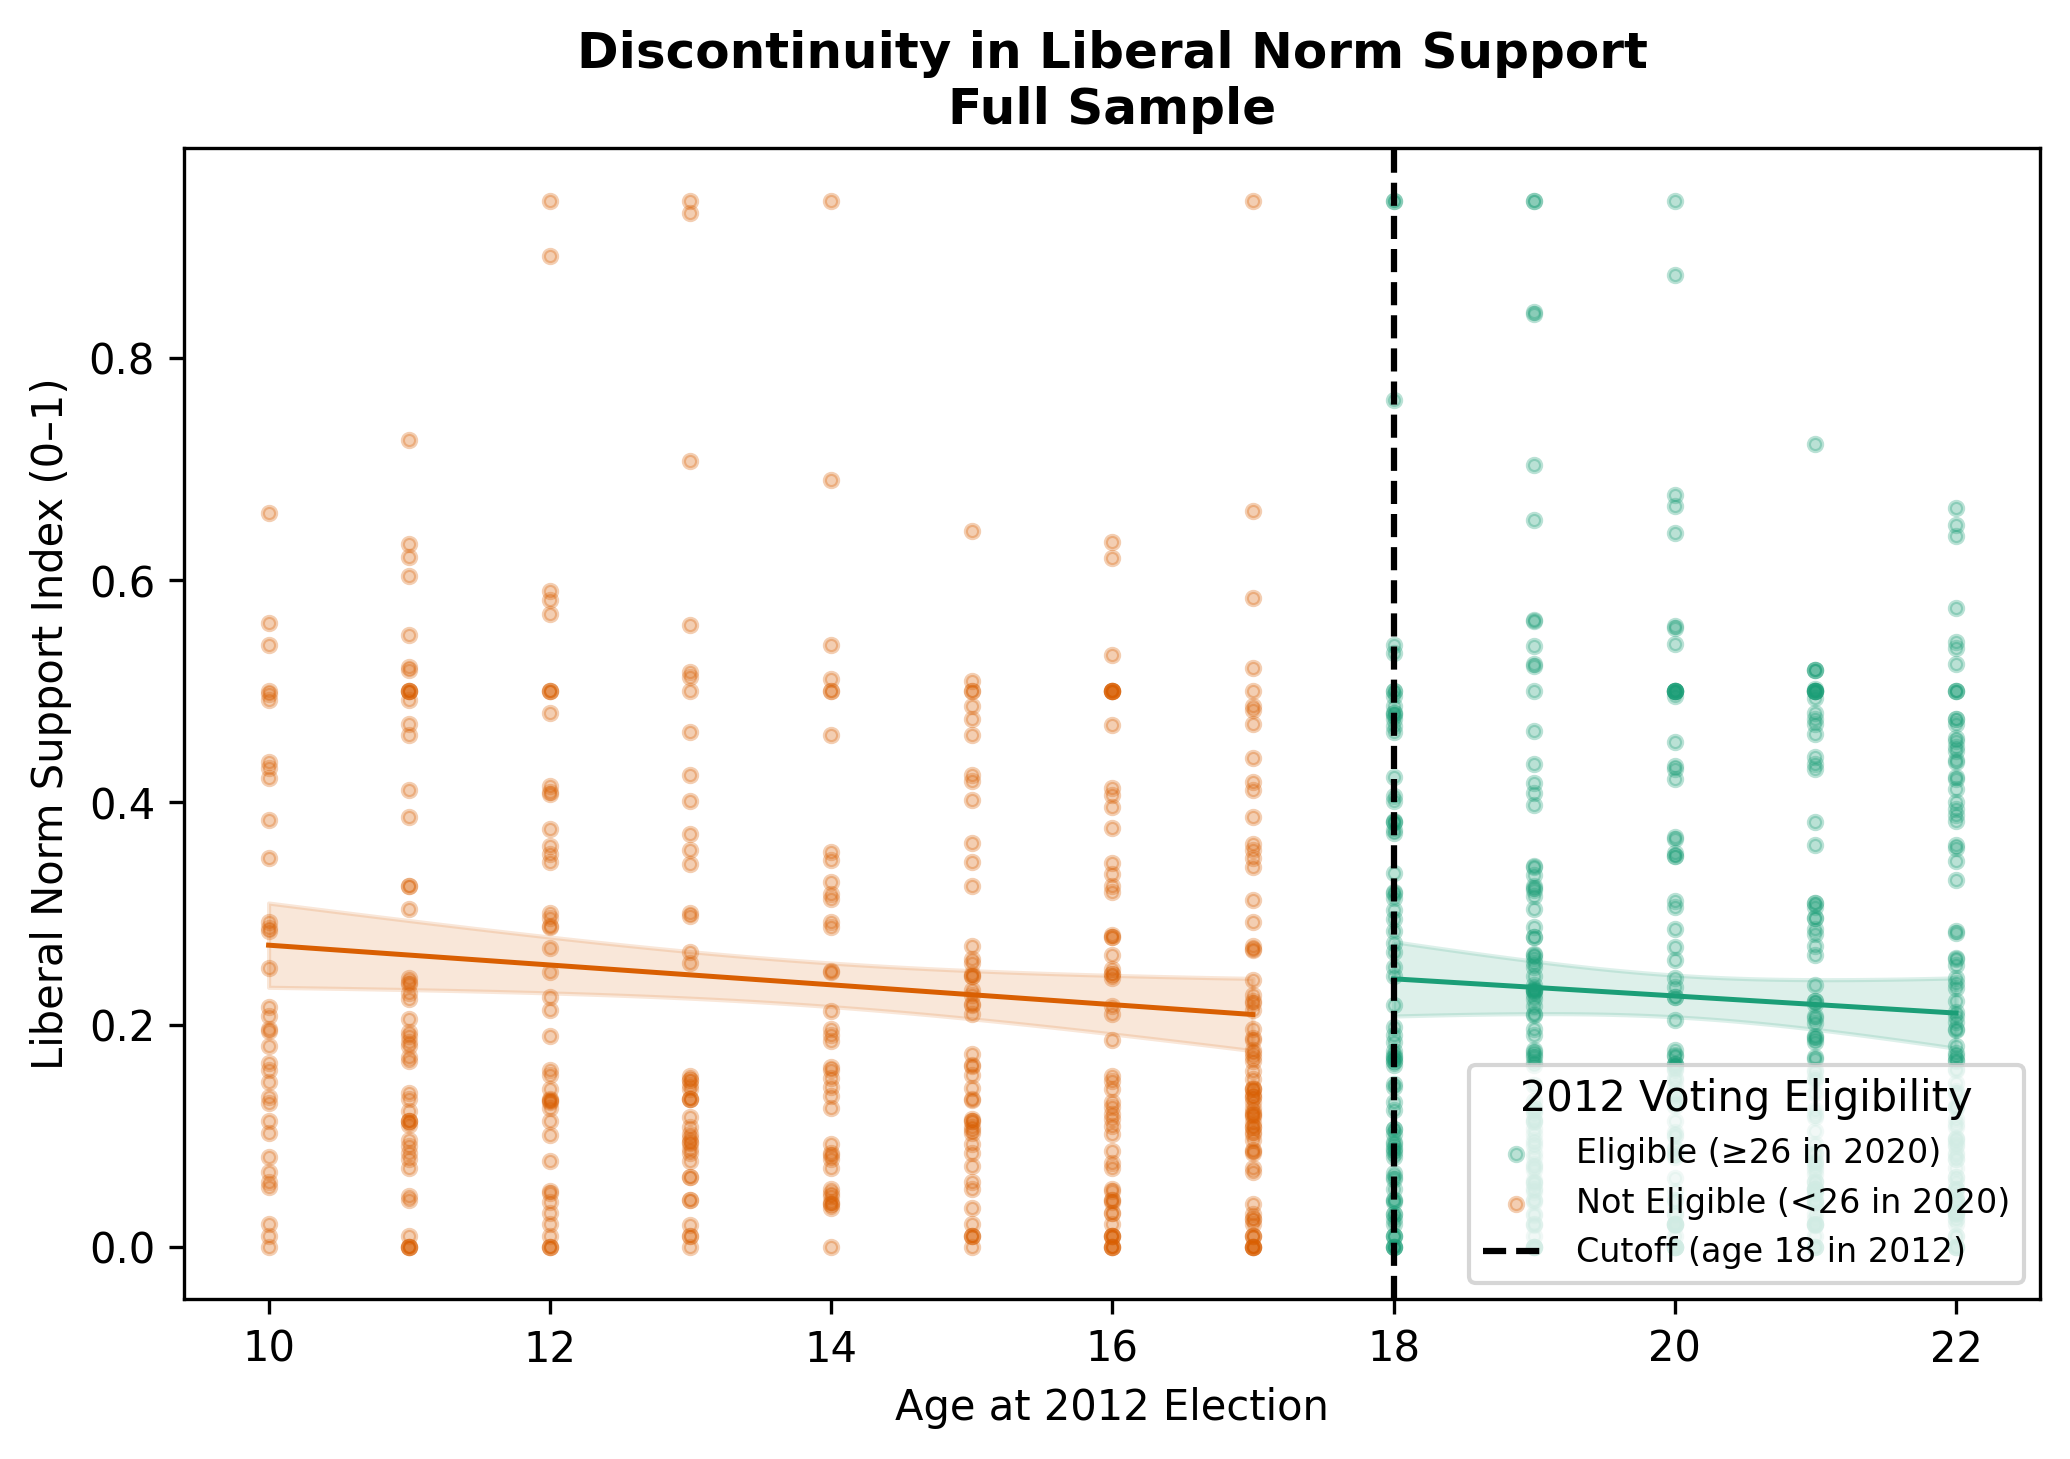
\includegraphics[width=9cm,height=\textheight,keepaspectratio]{images/discontinuityplot_full.png}

}

\caption{\label{fig-disfull}Discontinuity in Liberal Attitudes at the
Cutoff (Full Sample)}

\end{figure}%

There is no visually apparent discontinuity at the threshold for the
full sample. The confidence intervals on both sides of the cutoff
overlap substantially, and the fitted lines run smoothly through the
threshold without any clear jump. Figure~\ref{fig-dissubset} breaks this
down by partisanship subgroup.

\begin{figure}

\centering{

\pandocbounded{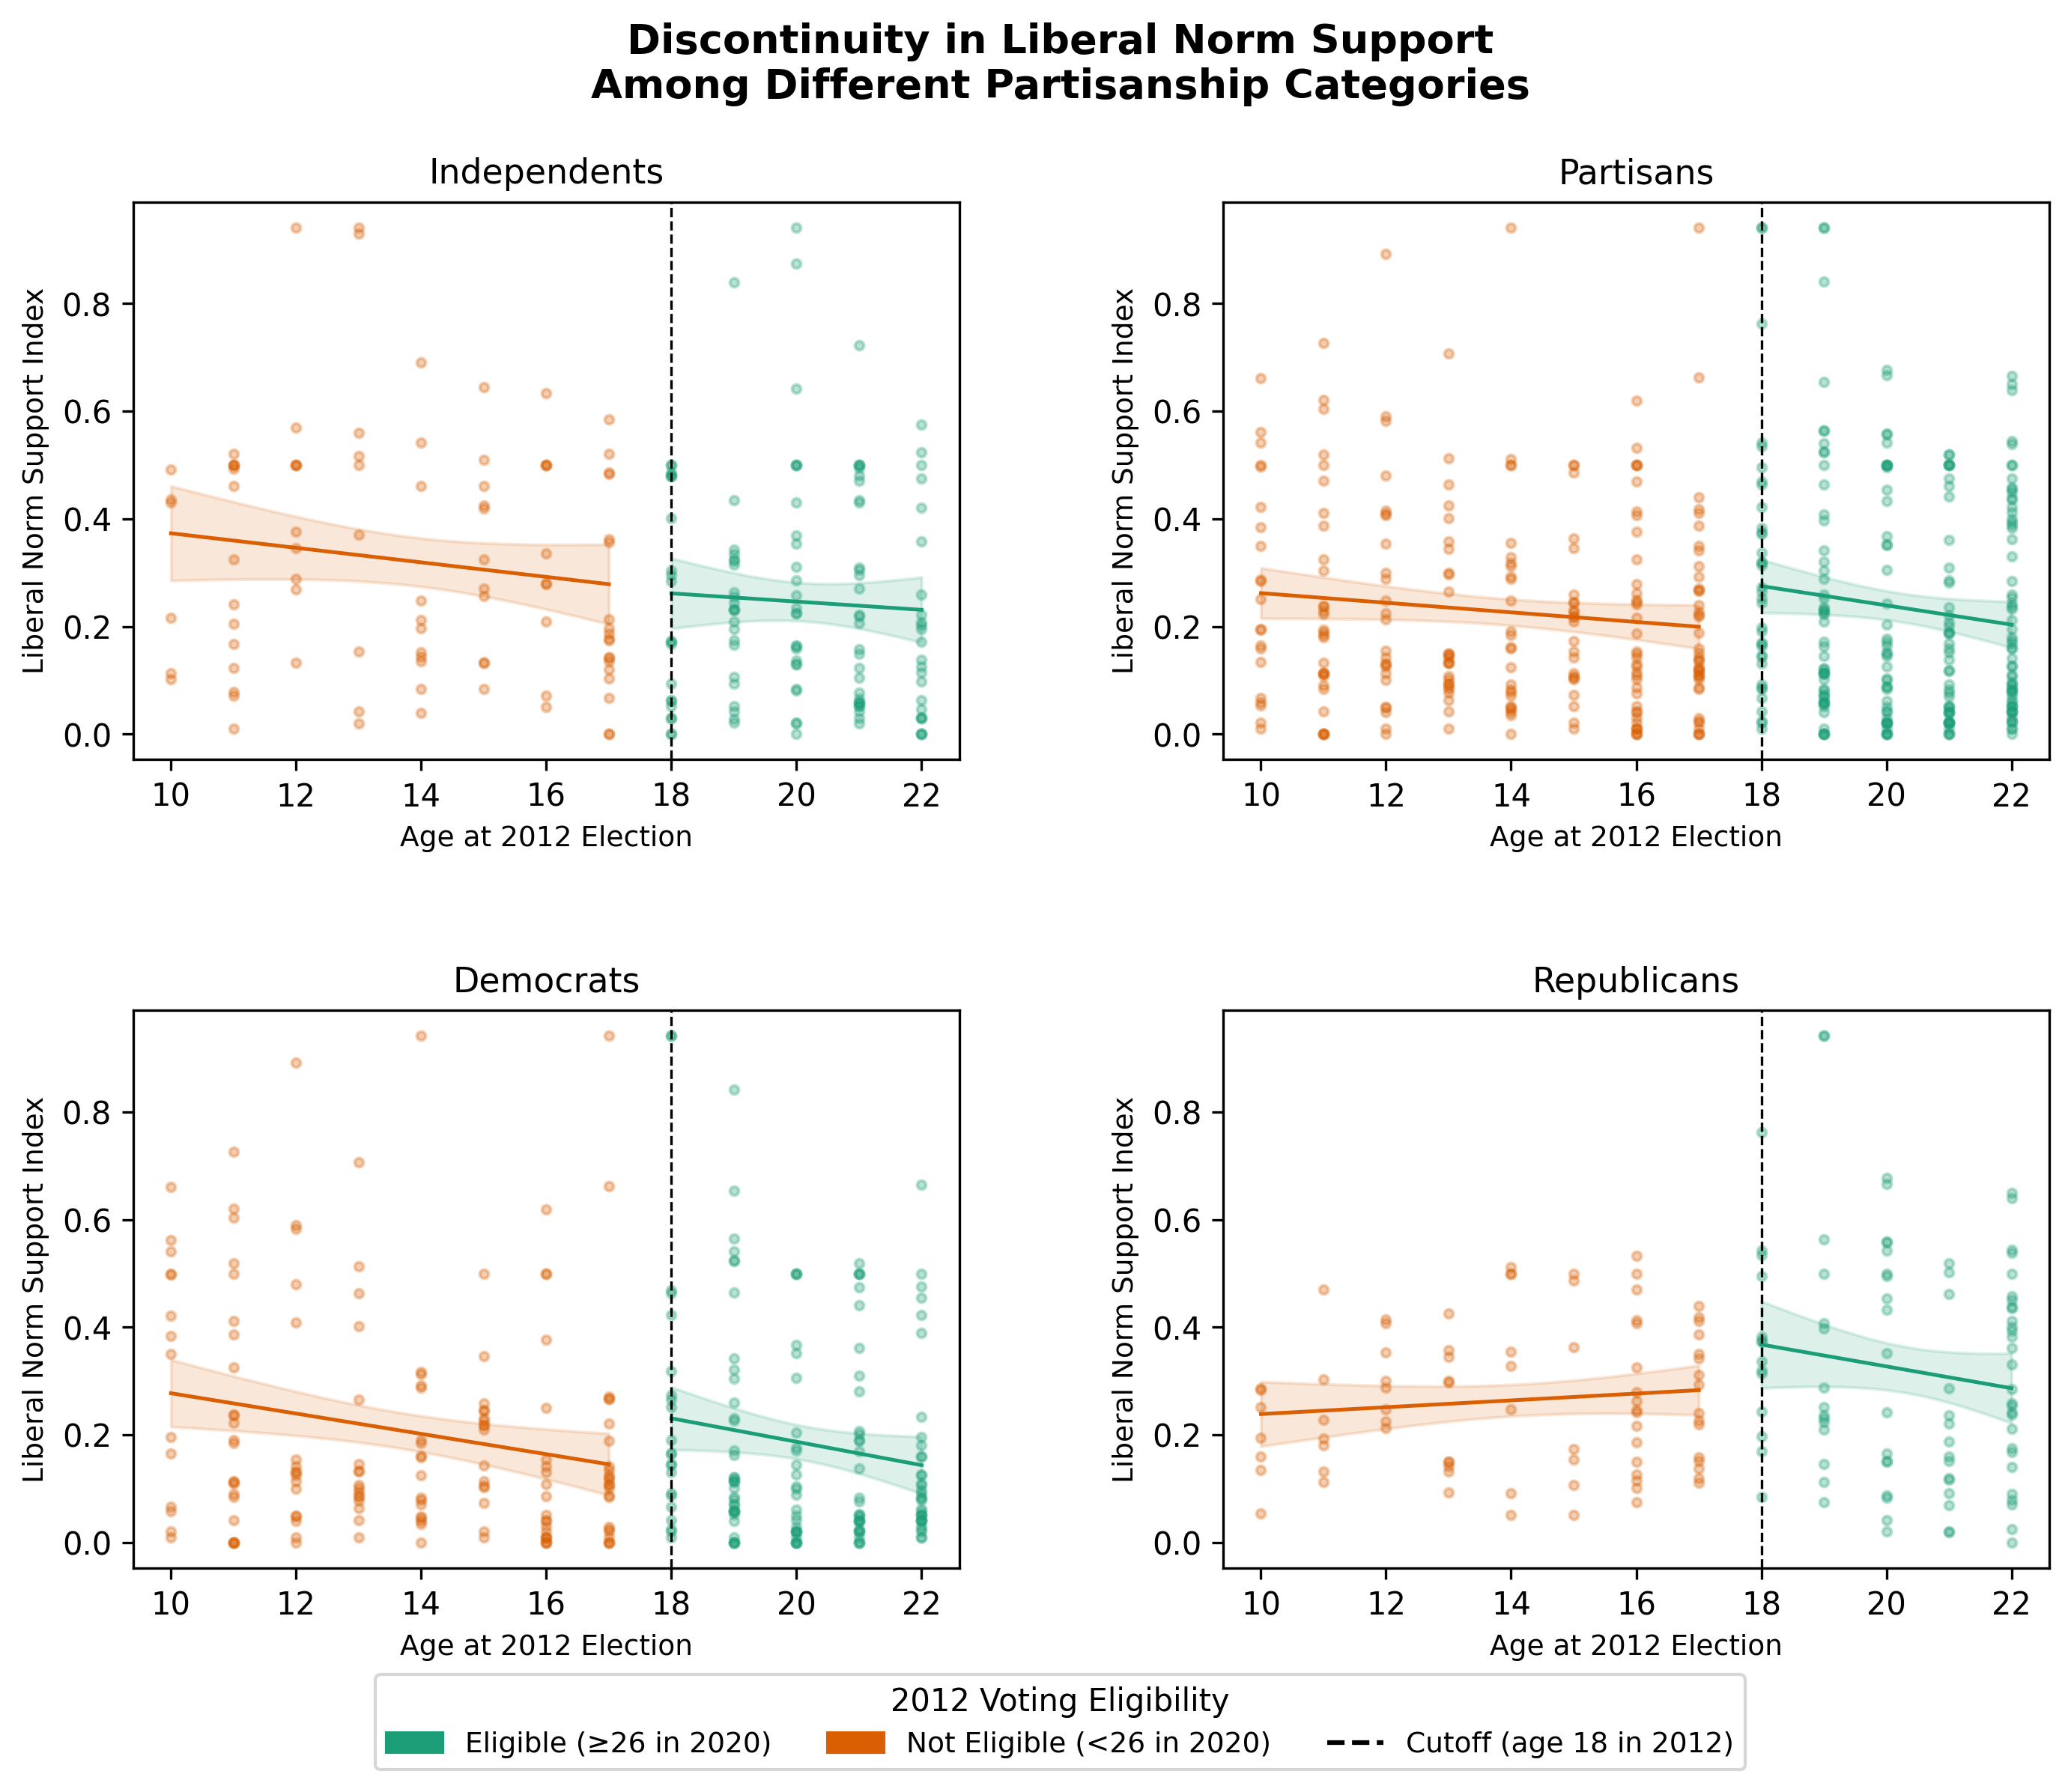
\includegraphics[keepaspectratio]{images/discontinuityplot_subgroups.png}}

}

\caption{\label{fig-dissubset}Discontinuity in Liberal Attitudes at the
Age-18 Cutoff (Partisanship Subgroups)}

\end{figure}%

The same pattern holds across all subgroups. Whether examining
independents, partisans, Democrats, or Republicans separately, no
visually compelling discontinuity is apparent at the threshold. In all
panels, the confidence intervals on both sides of the cutoff overlap,
consistent with a null result.

\subsection{RD Results}\label{rd-results}

Figure~\ref{fig-coefplot} presents the estimated treatment effects
(\(\tau\)) from the bias-corrected local linear RD models, with and
without controls, for each sample. All estimates are expressed on a 0--1
scale.

\begin{figure}

\centering{

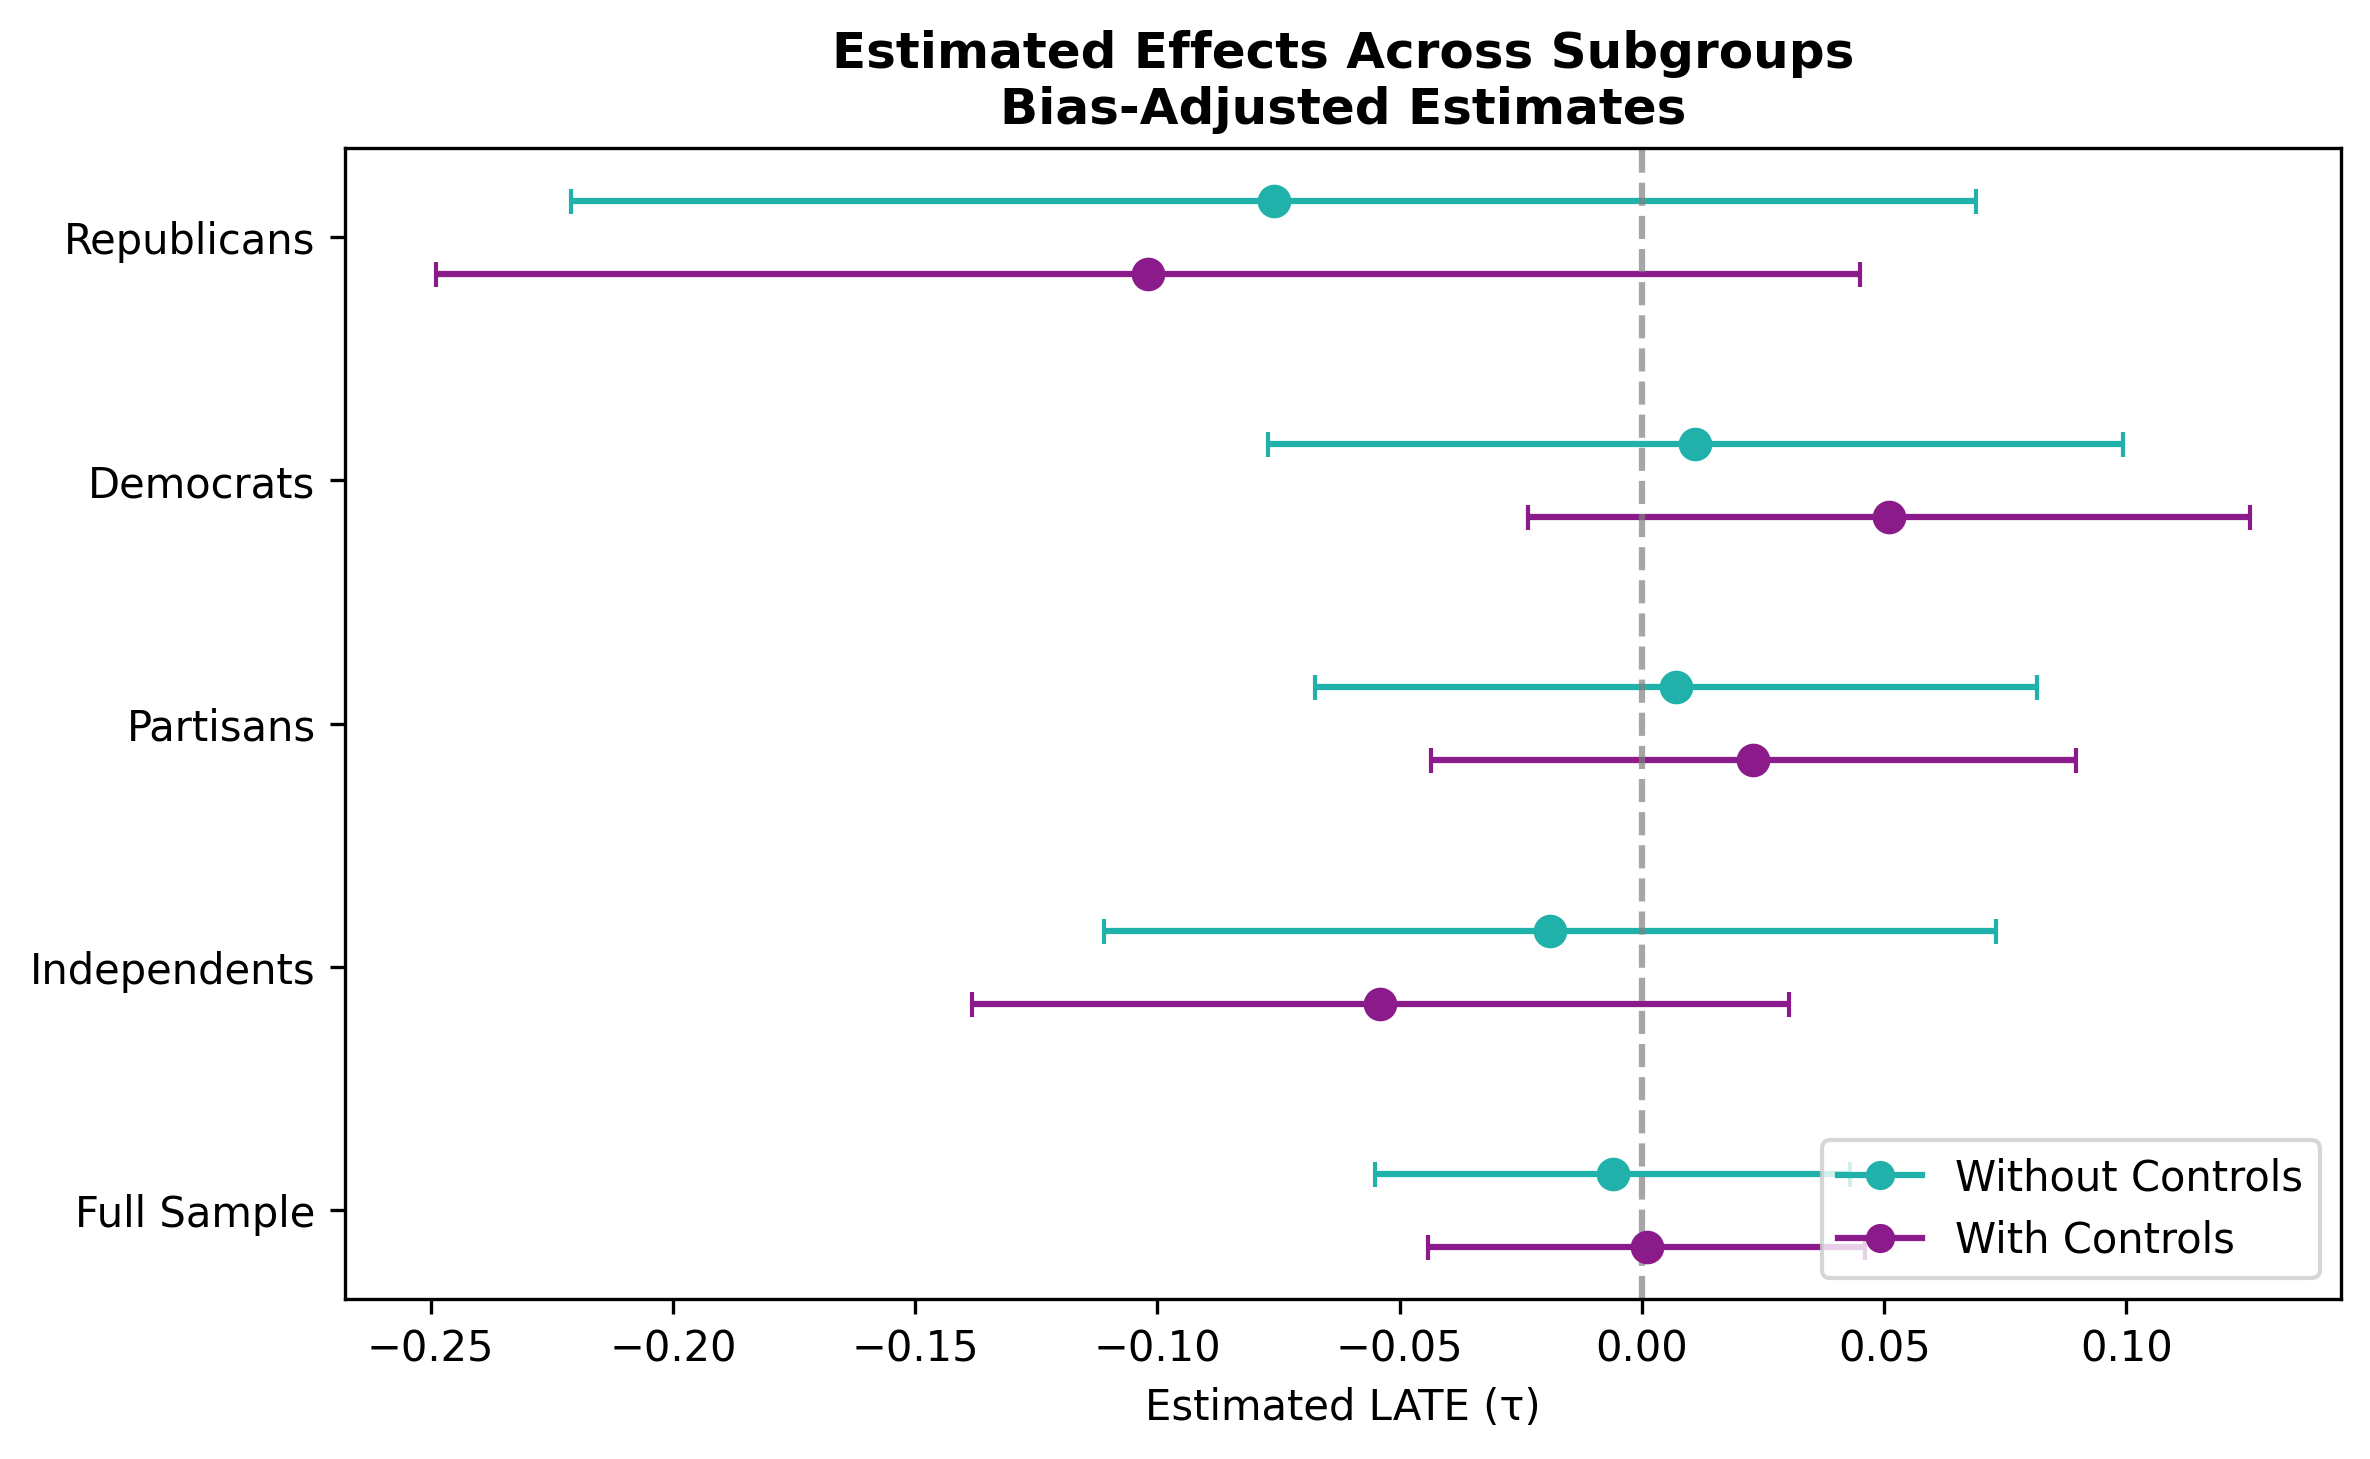
\includegraphics[width=12cm,height=\textheight,keepaspectratio]{images/coefplot_liberal.png}

}

\caption{\label{fig-coefplot}Points represent the bias-corrected
estimate of \(\tau\) at the cutoff, with horizontal lines indicating
95\% confidence intervals. A negative \(\tau\) indicates that 2016
first-time voters score lower on the liberalism index than 2012
first-time voters, consistent with H1. Separate estimates are shown for
the full sample and partisan subgroups, with and without controls for
education, income, and race.}

\end{figure}%

\subsubsection{H1: First-Time
Sensitivity}\label{h1-first-time-sensitivity}

For the full sample, the estimated discontinuity is small and
statistically insignificant in both the uncontrolled and controlled
models. There is no detectable causal effect of first-time voting
eligibility timing on liberal attitude scores at the threshold. The data
therefore provide no support for H1: coming of age during the 2016 Trump
election does not appear to produce measurably weaker liberal
commitments relative to those who first voted in 2012.

\subsubsection{H2: Non-Partisan
Insensitivity}\label{h2-non-partisan-insensitivity}

Among independents, \(\tau\) is small and statistically insignificant,
consistent with the expectation of H2 that politically unaffiliated
individuals would be less sensitive to the political context of their
democratic initiation. Among partisans, the estimate is likewise
insignificant, offering no evidence that partisan identifiers were more
affected by first-vote timing than the full sample. H2 therefore finds
no empirical support in these data.

\subsubsection{H3: Asymmetric
Sensitivity}\label{h3-asymmetric-sensitivity}

Separating partisans by party, the estimates for both Democrats and
Republicans are statistically insignificant across both specifications.
No asymmetric effect is detectable: Republican first-time voters do not
differ meaningfully from their slightly older counterparts in their
liberal attitude scores, nor do Democrats. H3 is not supported.

\subsection{Robustness Checks}\label{robustness-checks}

Given that the main estimates are null across all subgroups, the
robustness checks serve primarily to confirm stability rather than to
qualify significant findings. Figure~\ref{fig-coefplotrobust} presents
the three estimate types side by side.

\begin{figure}

\centering{

\pandocbounded{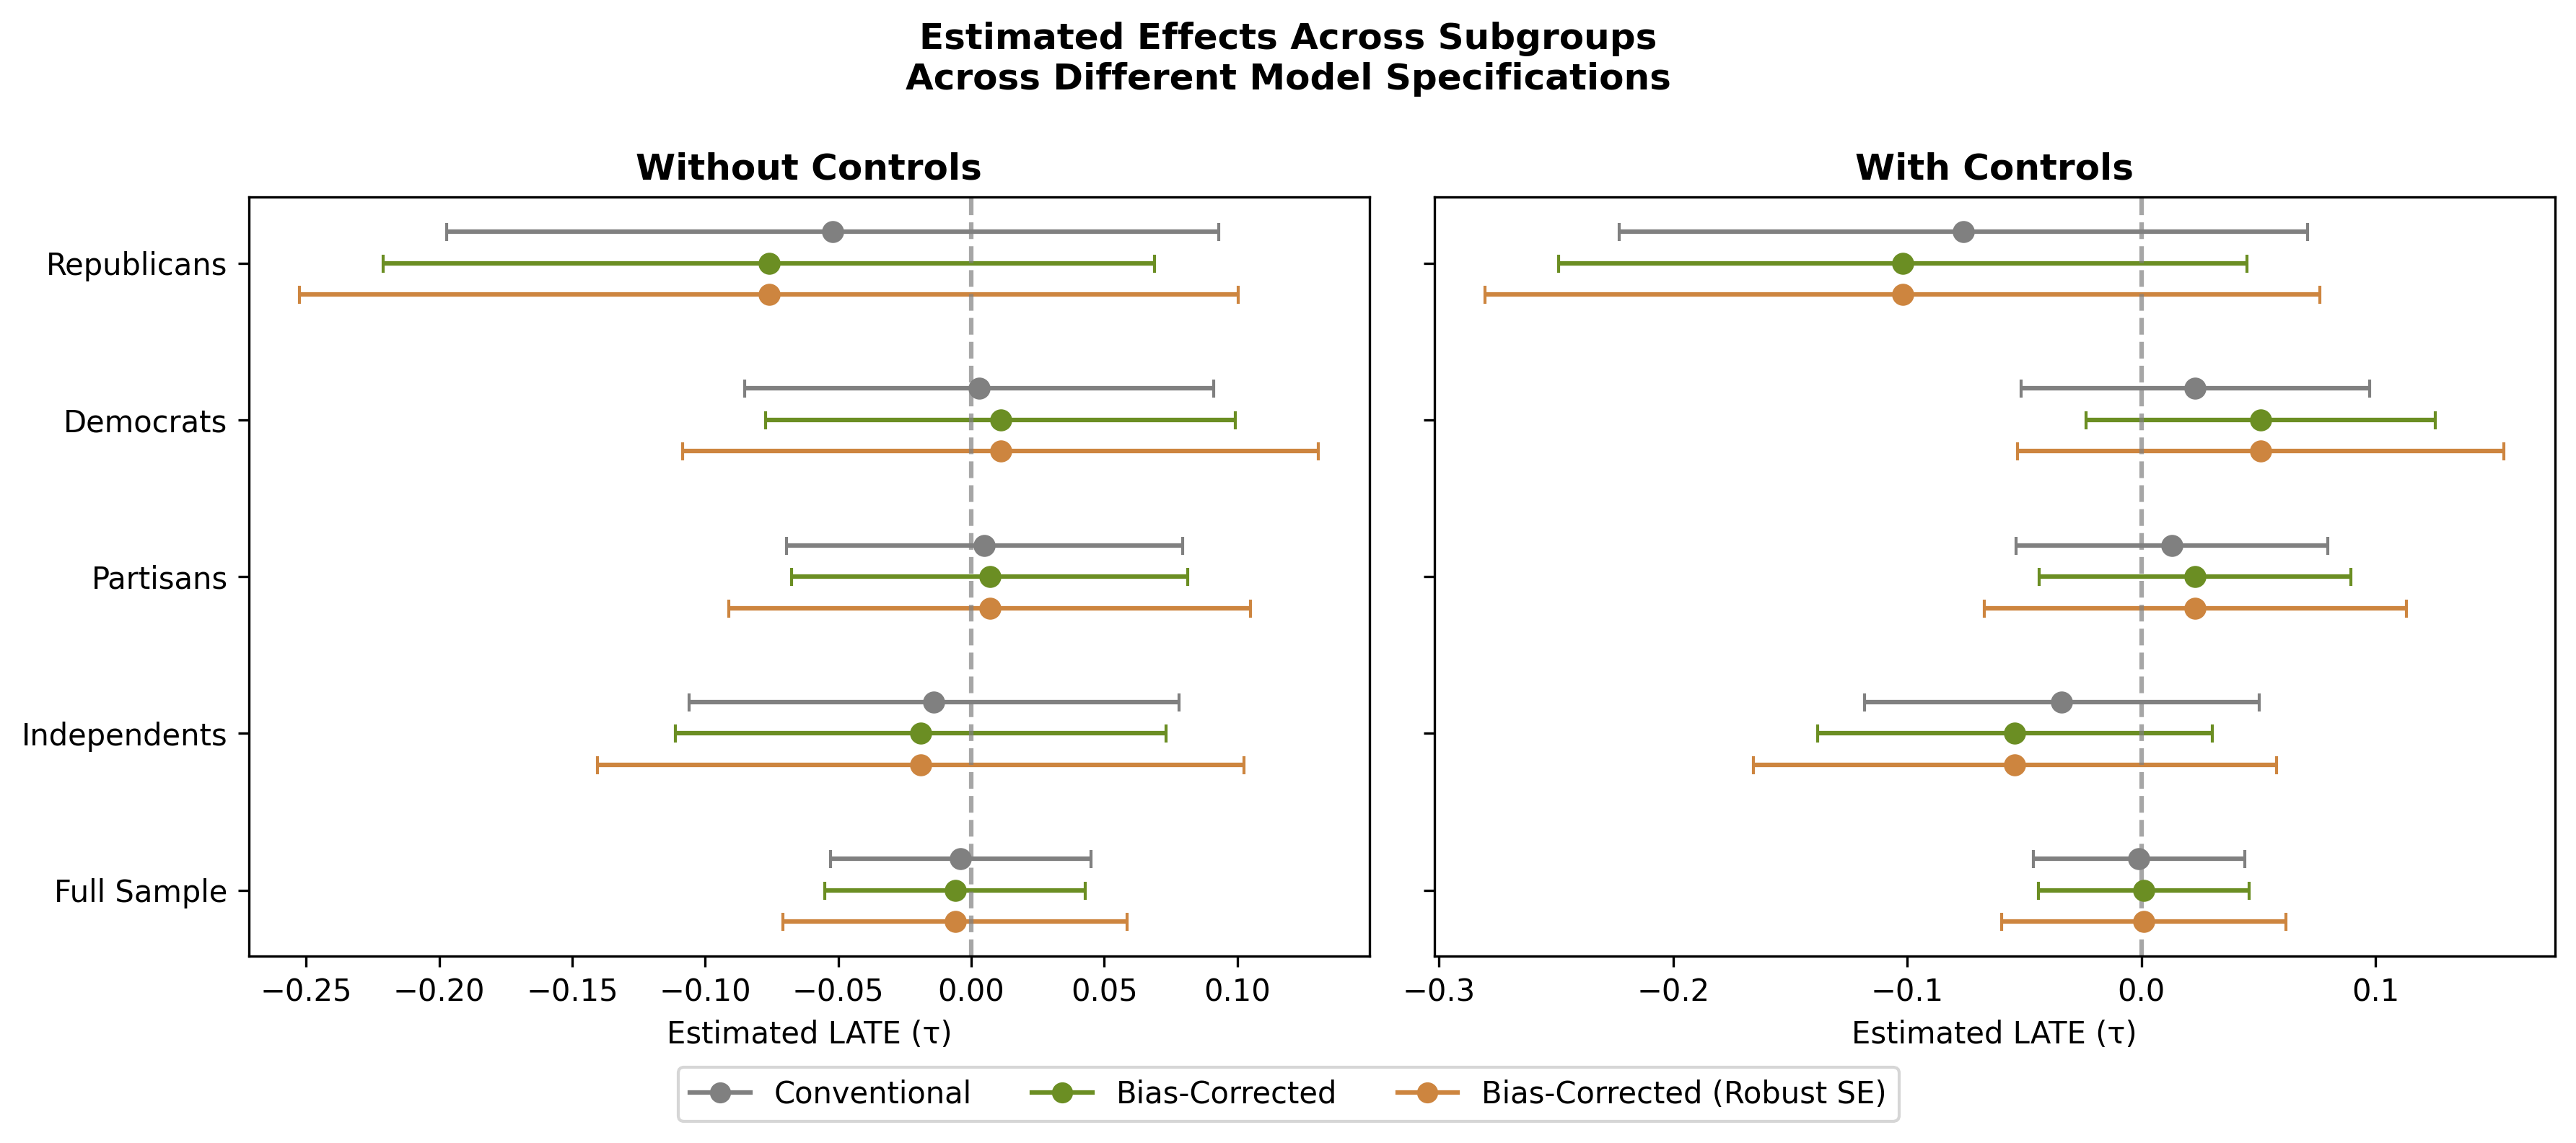
\includegraphics[keepaspectratio]{images/coefplot_robustness.png}}

}

\caption{\label{fig-coefplotrobust}Comparison of Estimate Types
(Conventional, Bias-Corrected, and Bias-Corrected with Robust Standard
Errors) across subgroups and model specifications.}

\end{figure}%

The null result is consistent across all three estimate types for every
subgroup, with and without controls. Figure~\ref{fig-robustness}
presents the bandwidth sensitivity, placebo cutoff, and polynomial
degree checks for the full Democrat subgroup, as an illustrative
case.\footnote{Robustness checks for the remaining subgroups are
  presented in the Appendix.}

\begin{figure}

\centering{

\pandocbounded{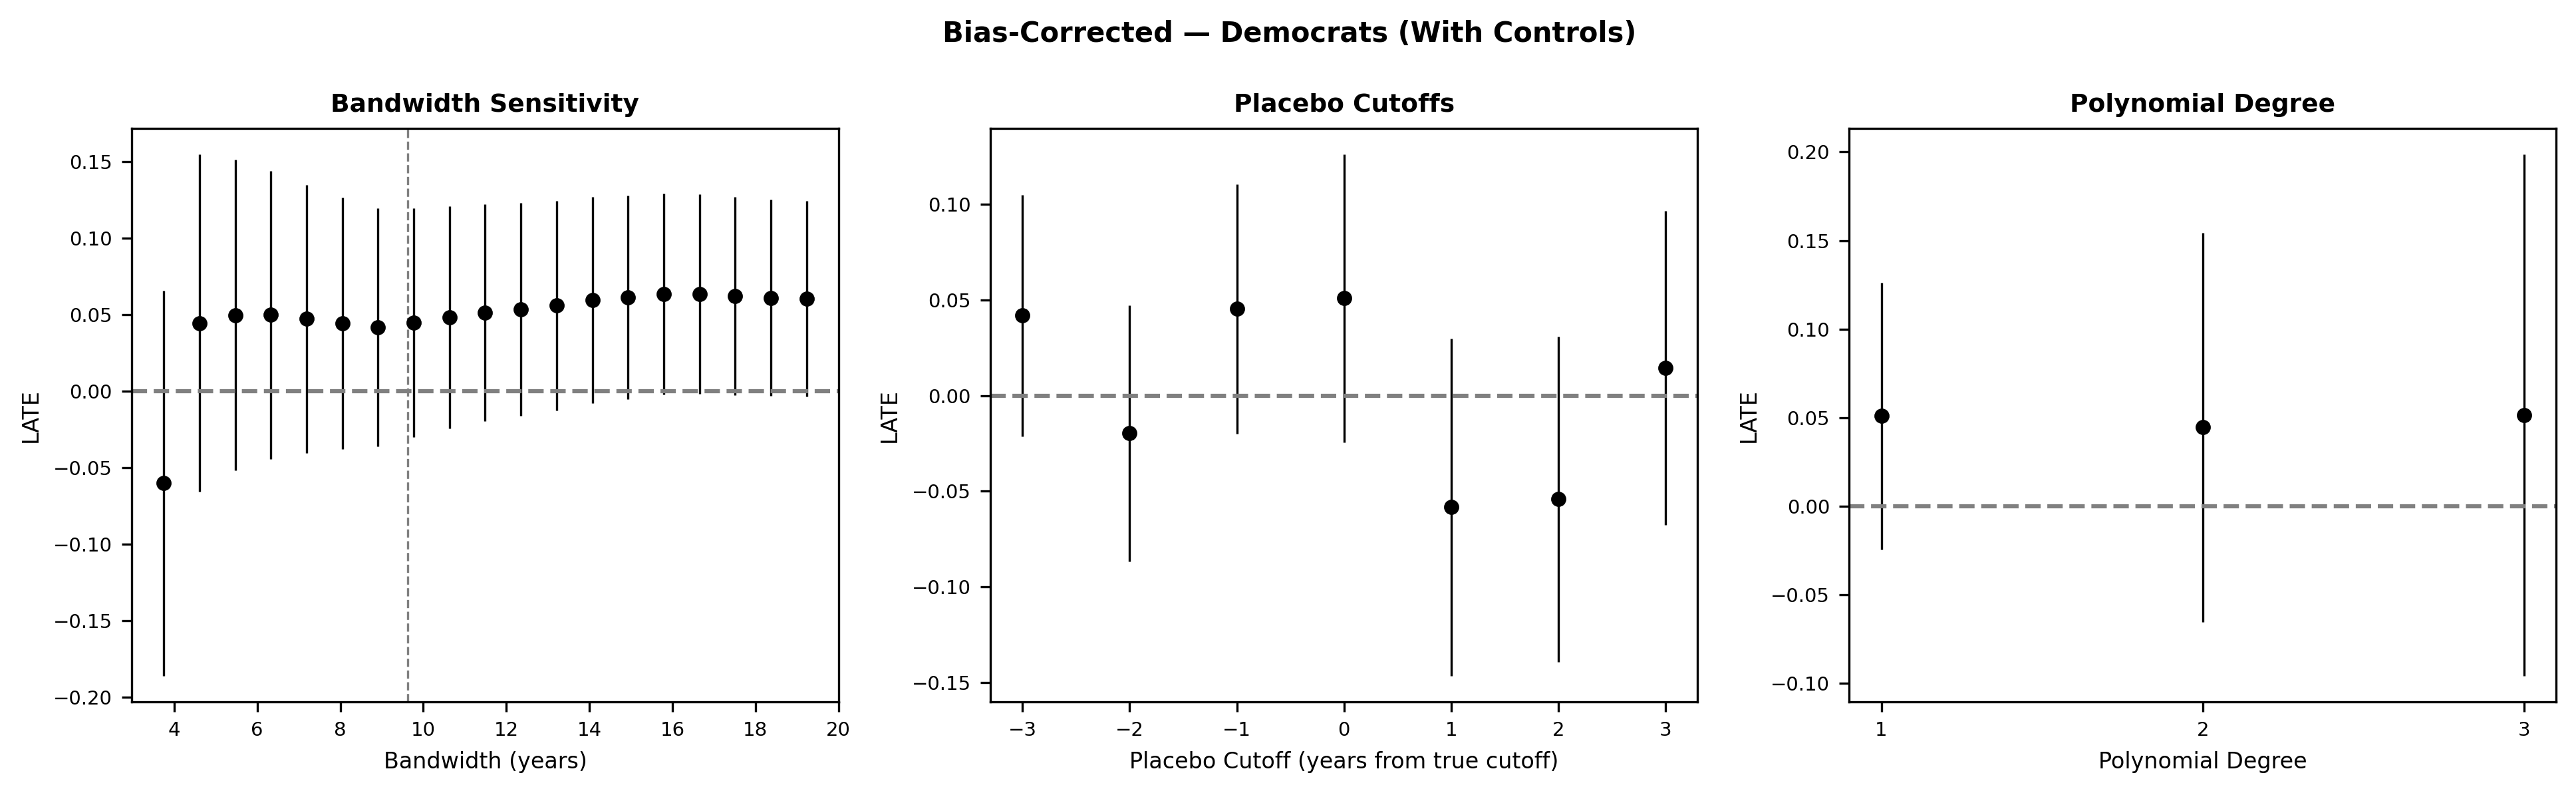
\includegraphics[keepaspectratio]{images/robustness_Democrats.png}}

}

\caption{\label{fig-robustness}Robustness Checks: Bandwidth Sensitivity,
Placebo Cutoffs, and Polynomial Degree (Democrats)}

\end{figure}%

Estimates remain consistently null across a wide range of bandwidths.
Placebo cutoffs at \(\pm 1\), \(\pm 2\), and \(\pm 3\) years from the
true threshold similarly yield insignificant results, suggesting that
the null finding at the true cutoff is not an artifact of the specific
threshold chosen. Results are also stable across polynomial degrees.
Taken together, the robustness checks reinforce the conclusion that
there is no detectable effect of first-vote timing on liberal democratic
attitudes in this sample.

\section{Conclusion}\label{conclusion-1}

This paper set out to ask whether coming of age during the 2016 Trump
election produced measurably weaker liberal democratic commitments.
Using a sharp RDD that compares those just eligible to vote in 2012 to
those who first voted in 2016, I find no statistically significant
discontinuity in liberal attitudes, neither in the full sample nor
across any partisan subgroup. These null results are stable across
alternative bandwidths, placebo cutoffs, and polynomial specifications.
Taken together, they suggest that political socialization during a
period of elite norm violation does not automatically translate into
weaker liberal commitments among those just entering the electorate.

These findings are notable in their own right. One possible
interpretation is that liberal democratic norms are more durable and
resistant to short-term contextual shocks than theories of
impressionable-years socialization might imply. Another is that the
mechanism connecting first-time voting context to democratic attitudes
is more complex, conditional, or delayed than the simple exposure
hypothesis tested here captures, perhaps requiring sustained exposure
over multiple electoral cycles rather than a single formative election.

Several avenues for future research follow directly from these
limitations. First, the present design relies on age measured in years
in the 2020 ANES, which introduces a non-trivial measurement margin
around the true eligibility cutoff. Future work using exact birth dates
(available in restricted-access versions of the ANES) would sharpen the
discontinuity considerably, potentially uncovering effects that are
obscured by the coarseness of the current running variable. Second, the
sample of first-time 2016 voters in the 2020 ANES is small relative to
the full sample, limiting statistical power. Replication using the 2024
ANES, or pooling across multiple survey waves, could improve precision
while also enabling an examination of whether the effects might change
due to exposure to the polarized contexts of the 2020 and 2024
presidential elections.Third, future research could examine whether the
null results are specific to the liberal norms dimension, or whether
they extend to electoral norms and attitudes toward democratic
institutions more broadly.

Finally, the interaction between political socialization and partisan
power status deserves closer attention: research on democratic hypocrisy
suggests that citizens apply different standards to democratic norms
depending on whether their party holds power
(\citeproc{ref-simonovits2022}{Simonovits, McCoy, and Littvay 2022};
\citeproc{ref-graham2020}{M. H. Graham and Svolik 2020}). Young voters
who came of age in 2016 experienced a Republican win whereas those who
first voted in 2020 experienced a contested Democratic win. Whether the
socialization effect differs depending on which party is in power at the
moment of political initiation, and how this interacts with the
respondent's own partisan identity, is a theoretically rich question
that warrants further study.

\newpage{}

\newpage{}

\section*{\texorpdfstring{\textbf{Bibliography}}{Bibliography}}\label{bibliography}
\addcontentsline{toc}{section}{\textbf{Bibliography}}

\phantomsection\label{refs}
\begin{CSLReferences}{1}{0}
\bibitem[\citeproctext]{ref-arceneaux2023}
Arceneaux, Kevin, and Rory Truex. 2023. {``Donald Trump and the Lie.''}
\emph{Perspectives on Politics} 21 (3): 863--79.
\url{https://doi.org/10.1017/S1537592722000901}.

\bibitem[\citeproctext]{ref-archer2023}
Archer, Allison M N. 2023. {``The Effects of Elite Attacks on Copartisan
Media: Evidence from Trump and Fox News.''} \emph{Public Opinion
Quarterly} 87 (4): 887--910. \url{https://doi.org/10.1093/poq/nfad042}.

\bibitem[\citeproctext]{ref-arnett2000}
Arnett, Jeffrey Jensen. 2000. {``Emerging Adulthood: A Theory of
Development from the Late Teens Through the Twenties.''} \emph{American
Psychologist} 55 (5): 469--80.
\url{https://doi.org/10.1037/0003-066X.55.5.469}.

\bibitem[\citeproctext]{ref-bakker2020}
Bakker, Bert N., Yphtach Lelkes, and Ariel Malka. 2020. {``Understanding
Partisan Cue Receptivity: Tests of Predictions from the Bounded
Rationality and Expressive Utility Perspectives.''} \emph{The Journal of
Politics} 82 (3): 1061--77. \url{https://doi.org/10.1086/707616}.

\bibitem[\citeproctext]{ref-banda2021}
Banda, Kevin K. 2021. {``Issue Ownership Cues and Candidate Support.''}
\emph{Party Politics} 27 (3): 552--64.
\url{https://doi.org/10.1177/1354068819869901}.

\bibitem[\citeproctext]{ref-bartels2020}
Bartels, Larry M. 2020. {``Ethnic Antagonism Erodes Republicans{'}
Commitment to Democracy.''} \emph{Proceedings of the National Academy of
Sciences} 117 (37): 22752--59.
\url{https://doi.org/10.1073/pnas.2007747117}.

\bibitem[\citeproctext]{ref-bekafigo2019}
Bekafigo, Marija A., Elena V. Stepanova, Brian A. Eiler, Kenji Noguchi,
and Kathleen L. Ramsey. 2019. {``The Effect of Group Polarization on
Opposition to Donald Trump.''} \emph{Political Psychology} 40 (5):
1163--78. \url{https://www.jstor.org/stable/45204110}.

\bibitem[\citeproctext]{ref-bellucci2020}
Bellucci, Davide, Giulia Fuochi, and Pierluigi Conzo. 2020. {``Childhood
Exposure to the Second World War and Financial Risk Taking in Adult
Life.''} \emph{Journal of Economic Psychology}, The impact of life
experiences on risk taking, 79 (August): 102196.
\url{https://doi.org/10.1016/j.joep.2019.102196}.

\bibitem[\citeproctext]{ref-boxell2024}
Boxell, Levi, Matthew Gentzkow, and Jesse M. Shapiro. 2024.
{``Cross-Country Trends in Affective Polarization.''} \emph{The Review
of Economics and Statistics} 106 (2): 557--65.
\url{https://doi.org/10.1162/rest_a_01160}.

\bibitem[\citeproctext]{ref-brader2012}
Brader, Ted, and Joshua A. Tucker. 2012. {``Following the Party's Lead:
Party Cues, Policy Opinion, and the Power of Partisanship in Three
Multiparty Systems.''}
\url{https://www.ingentaconnect.com/content/cuny/cp/2012/00000044/00000004/art00003}.

\bibitem[\citeproctext]{ref-braley2023}
Braley, Alia, Gabriel S. Lenz, Dhaval Adjodah, Hossein Rahnama, and Alex
Pentland. 2023. {``Why voters who value democracy participate in
democratic backsliding.''} \emph{Nature Human Behaviour} 7 (8):
1282--93. \url{https://doi.org/10.1038/s41562-023-01594-w}.

\bibitem[\citeproctext]{ref-broockman2023}
Broockman, David E., Joshua L. Kalla, and Sean J. Westwood. 2023.
{``Does Affective Polarization Undermine Democratic Norms or
Accountability? Maybe Not.''} \emph{American Journal of Political
Science} 67 (3): 808--28. \url{https://doi.org/10.1111/ajps.12719}.

\bibitem[\citeproctext]{ref-carraro2011}
Carraro, Luciana, Luigi Castelli, and Claudia Macchiella. 2011. {``The
Automatic Conservative: Ideology-Based Attentional Asymmetries in the
Processing of Valenced Information.''} \emph{PLOS ONE} 6 (11): e26456.
\url{https://doi.org/10.1371/journal.pone.0026456}.

\bibitem[\citeproctext]{ref-cassese2021}
Cassese, Erin C. 2021. {``Partisan Dehumanization in American
Politics.''} \emph{Political Behavior} 43 (1): 29--50.
\url{https://doi.org/10.1007/s11109-019-09545-w}.

\bibitem[\citeproctext]{ref-claassen2020}
Claassen, Christopher. 2020. {``Does Public Support Help Democracy
Survive?''} \emph{American Journal of Political Science} 64 (1):
118--34. \url{https://doi.org/10.1111/ajps.12452}.

\bibitem[\citeproctext]{ref-claassen2025}
Claassen, Christopher, Kathrin Ackermann, Eri Bertsou, Lucas Borba, Ryan
E. Carlin, Amnon Cavari, Sirianne Dahlum, et al. 2025.
{``Conceptualizing and Measuring Support for Democracy: A New
Approach.''} \emph{Comparative Political Studies} 58 (6): 1171--98.
\url{https://doi.org/10.1177/00104140241259458}.

\bibitem[\citeproctext]{ref-claassen2023}
Claassen, Christopher, and Pedro C Magalhães. 2023. {``Public Support
for Democracy in the United States Has Declined Generationally.''}
\emph{Public Opinion Quarterly} 87 (3): 719--32.
\url{https://doi.org/10.1093/poq/nfad039}.

\bibitem[\citeproctext]{ref-clayton2021}
Clayton, Katherine, Nicholas T. Davis, Brendan Nyhan, Ethan Porter,
Timothy J. Ryan, and Thomas J. Wood. 2021. {``Elite Rhetoric Can
Undermine Democratic Norms.''} \emph{Proceedings of the National Academy
of Sciences} 118 (23): e2024125118.
\url{https://doi.org/10.1073/pnas.2024125118}.

\bibitem[\citeproctext]{ref-coppedge2016}
Coppedge, Michael, Staffan Lindberg, Svend-Erik Skaaning, and Jan
Teorell. 2016. {``Measuring High Level Democratic Principles Using the
v-Dem Data.''} \emph{International Political Science Review} 37 (5):
580--93. \url{https://doi.org/10.1177/0192512115622046}.

\bibitem[\citeproctext]{ref-cremer2023}
Cremer, Tobias. 2023. {``A Europeanisation of American Politics?:
Trumpism and the Populist Radical Right in the United States.''}
\emph{Journal of Language and Politics} 22 (3): 396414.
\url{https://doi.org/10.1075/jlp.22135.cre}.

\bibitem[\citeproctext]{ref-dahl1971}
Dahl, Robert Alan. 1971. \emph{Polyarchy: Participation and Opposition}.
Yale University Press.

\bibitem[\citeproctext]{ref-dickson2025}
Dickson, Zachary P., and Sara B. Hobolt. 2025. {``Elite Cues and
Noncompliance.''} \emph{American Political Science Review} 119 (2):
870--86. \url{https://doi.org/10.1017/S0003055424000741}.

\bibitem[\citeproctext]{ref-dinas2012}
Dinas, Elias. 2012. {``The Formation of Voting Habits.''} \emph{Journal
of Elections, Public Opinion and Parties} 22 (4): 431--56.
\url{https://doi.org/10.1080/17457289.2012.718280}.

\bibitem[\citeproctext]{ref-dinas2013}
---------. 2013. {``Opening {``}Openness to Change{''}: Political Events
and the Increased Sensitivity of Young Adults.''} \emph{Political
Research Quarterly} 66 (4): 868--82.
\url{https://doi.org/10.1177/1065912913475874}.

\bibitem[\citeproctext]{ref-dodd2012}
Dodd, Michael D., Amanda Balzer, Carly M. Jacobs, Michael W.
Gruszczynski, Kevin B. Smith, and John R. Hibbing. 2012. {``The
Political Left Rolls with the Good and the Political Right Confronts the
Bad: Connecting Physiology and Cognition to Preferences.''}
\emph{Philosophical Transactions of the Royal Society B: Biological
Sciences} 367 (1589): 640--49.
\url{https://doi.org/10.1098/rstb.2011.0268}.

\bibitem[\citeproctext]{ref-druckman2024}
Druckman, James N. 2024. {``How to Study Democratic Backsliding.''}
\emph{Political Psychology} 45 (S1): 3--42.
\url{https://doi.org/10.1111/pops.12942}.

\bibitem[\citeproctext]{ref-druckman2023}
Druckman, James N., Donald P. Green, and Shanto Iyengar. 2023. {``Does
Affective Polarization Contribute to Democratic Backsliding in
America?''} \emph{The ANNALS of the American Academy of Political and
Social Science} 708 (1): 137--63.
\url{https://doi.org/10.1177/00027162241228952}.

\bibitem[\citeproctext]{ref-foa2016}
Foa, Roberto Stefan, and Yascha Mounk. 2016. {``The Danger of
Deconsolidation: The Democratic Disconnect.''} \emph{Journal of
Democracy} 27 (3): 5--17.
\url{https://muse.jhu.edu/pub/1/article/623602}.

\bibitem[\citeproctext]{ref-fossati2022}
Fossati, Diego, Burhanuddin Muhtadi, and Eve Warburton. 2022. {``Why
Democrats Abandon Democracy: Evidence from Four Survey Experiments.''}
\emph{Party Politics} 28 (3): 554--66.
\url{https://doi.org/10.1177/1354068821992488}.

\bibitem[\citeproctext]{ref-franklin2004}
Franklin, Mark N. 2004. \emph{Voter Turnout and the Dynamics of
Electoral Competition in Established Democracies Since 1945}. Cambridge:
Cambridge University Press.
\url{https://doi.org/10.1017/CBO9780511616884}.

\bibitem[\citeproctext]{ref-frederiksen2022a}
Frederiksen, Kristian Vrede Skaaning. 2022. {``Does Competence Make
Citizens Tolerate Undemocratic Behavior?''} \emph{American Political
Science Review} 116 (3): 1147--53.
\url{https://doi.org/10.1017/S0003055422000119}.

\bibitem[\citeproctext]{ref-fuller2025}
Fuller, Sam, Nicolás de la Cerda, and Jack T. Rametta. 2025. {``Affect,
Not Ideology: The Heterogeneous Effects of Partisan Cues on Policy
Support.''} \emph{Political Behavior}, March.
\url{https://doi.org/10.1007/s11109-025-10030-w}.

\bibitem[\citeproctext]{ref-ghitza2023}
Ghitza, Yair, Andrew Gelman, and Jonathan Auerbach. 2023. {``The Great
Society, Reagan's Revolution, and Generations of Presidential Voting.''}
\emph{American Journal of Political Science} 67 (3): 520--37.
\url{https://doi.org/10.1111/ajps.12713}.

\bibitem[\citeproctext]{ref-gidengil2022}
Gidengil, Elisabeth, Dietlind Stolle, and Olivier Bergeron-Boutin. 2022.
{``The Partisan Nature of Support for Democratic Backsliding: A
Comparative Perspective.''} \emph{European Journal of Political
Research} 61 (4): 901--29.
\url{https://doi.org/10.1111/1475-6765.12502}.

\bibitem[\citeproctext]{ref-graham2012}
Graham, Jesse, Brian A. Nosek, and Jonathan Haidt. 2012. {``The Moral
Stereotypes of Liberals and Conservatives: Exaggeration of Differences
Across the Political Spectrum.''} \emph{PLOS ONE} 7 (12): e50092.
\url{https://doi.org/10.1371/journal.pone.0050092}.

\bibitem[\citeproctext]{ref-graham2020}
Graham, Matthew H., and Milan W. Svolik. 2020. {``Democracy in America?
Partisanship, Polarization, and the Robustness of Support for Democracy
in the United States.''} \emph{American Political Science Review} 114
(2): 392409. \url{https://doi.org/10.1017/S0003055420000052}.

\bibitem[\citeproctext]{ref-grillo2023}
Grillo, Edoardo, and Carlo Prato. 2023. {``Reference Points and
Democratic Backsliding.''} \emph{American Journal of Political Science}
67 (1): 71--88. \url{https://doi.org/10.1111/ajps.12672}.

\bibitem[\citeproctext]{ref-grossman2022}
Grossman, Guy, Dorothy Kronick, Matthew Levendusky, and Marc Meredith.
2022. {``The Majoritarian Threat to Liberal Democracy.''} \emph{Journal
of Experimental Political Science} 9 (1): 36--45.
\url{https://doi.org/10.1017/XPS.2020.44}.

\bibitem[\citeproctext]{ref-holliday2024}
Holliday, Derek E., Shanto Iyengar, Yphtach Lelkes, and Sean J.
Westwood. 2024. {``Uncommon and Nonpartisan: Antidemocratic Attitudes in
the American Public.''} \emph{Proceedings of the National Academy of
Sciences} 121 (13): e2313013121.
\url{https://doi.org/10.1073/pnas.2313013121}.

\bibitem[\citeproctext]{ref-inbar2009}
Inbar, Yoel, Pizarro ,David A., and Paul and Bloom. 2009.
{``Conservatives Are More Easily Disgusted Than Liberals.''}
\emph{Cognition and Emotion} 23 (4): 714--25.
\url{https://doi.org/10.1080/02699930802110007}.

\bibitem[\citeproctext]{ref-iyengar2019}
Iyengar, Shanto, Yphtach Lelkes, Matthew Levendusky, Neil Malhotra, and
Sean J. Westwood. 2019. {``The Origins and Consequences of Affective
Polarization in the United States.''} \emph{Annual Review of Political
Science} 22 (Volume 22, 2019): 129--46.
\url{https://doi.org/10.1146/annurev-polisci-051117-073034}.

\bibitem[\citeproctext]{ref-iyengar2015}
Iyengar, Shanto, and Sean J. Westwood. 2015. {``Fear and Loathing Across
Party Lines: New Evidence on Group Polarization.''} \emph{American
Journal of Political Science} 59 (3): 690--707.
\url{https://doi.org/10.1111/ajps.12152}.

\bibitem[\citeproctext]{ref-jacob2025}
Jacob, Marc S. 2025. {``Citizen Support for Democracy, Anti-Pluralist
Parties in Power and Democratic Backsliding.''} \emph{European Journal
of Political Research} 64 (1): 348--73.
\url{https://doi.org/10.1111/1475-6765.12703}.

\bibitem[\citeproctext]{ref-jennings2014}
Jennings, M. Kent, and Richard G. Niemi. 2014. \emph{Generations and
Politics: A Panel Study of Young Adults and Their Parents}. Princeton
University Press.

\bibitem[\citeproctext]{ref-joel2014}
Joel, Samantha, Caitlin M. Burton, and Jason E. Plaks. 2014.
{``Conservatives Anticipate and Experience Stronger Emotional Reactions
to Negative Outcomes.''} \emph{Journal of Personality} 82 (1): 32--43.
\url{https://doi.org/10.1111/jopy.12031}.

\bibitem[\citeproctext]{ref-kaufman2019}
Kaufman, Robert R., and Stephan Haggard. 2019. {``Democratic decline in
the United States: What can we learn from middle-income backsliding?''}
\emph{Perspectives on Politics} 17 (2): 417--32.
\url{https://doi.org/10.1017/S1537592718003377}.

\bibitem[\citeproctext]{ref-kesternich2020}
Kesternich, Iris, James P. Smith, Joachim K. Winter, and Maximiliane
Hörl. 2020. {``Early-Life Circumstances Predict Measures of Trust Among
Adults: Evidence from Hunger Episodes in Post-War Germany.''} \emph{The
Scandinavian Journal of Economics} 122 (1): 280--305.
\url{https://doi.org/10.1111/sjoe.12329}.

\bibitem[\citeproctext]{ref-kingzette2021}
Kingzette, Jon, James N Druckman, Samara Klar, Yanna Krupnikov, Matthew
Levendusky, and John Barry Ryan. 2021. {``How Affective Polarization
Undermines Support for Democratic Norms.''} \emph{Public Opinion
Quarterly} 85 (2): 663--77. \url{https://doi.org/10.1093/poq/nfab029}.

\bibitem[\citeproctext]{ref-krishnarajan2023}
Krishnarajan, Suthan. 2023. {``Rationalizing Democracy: The Perceptual
Bias and (Un)Democratic Behavior.''} \emph{American Political Science
Review} 117 (2): 474--96.
\url{https://doi.org/10.1017/S0003055422000806}.

\bibitem[\citeproctext]{ref-luecken2010}
Luecken, Linda J., and Jenna L. Gress. 2010. {``Early Adversity and
Resilience in Emerging Adulthood.''} In, 238--57. New York, NY, US: The
Guilford Press.

\bibitem[\citeproctext]{ref-magleby2011}
Magleby, David B., Candice J. Nelson, and Mark C. Westlye. 2011. {``The
Myth of the Independent Voter Revisited.''} \emph{Facing the Challenge
of Democracy: Explorations in the Analysis of Public Opinion and
Political Participation}, 238--63.

\bibitem[\citeproctext]{ref-mandel2014}
Mandel, David R., and Philip Omorogbe. 2014. {``Political Differences in
Past, Present, and Future Life Satisfaction: Republicans Are More
Sensitive Than Democrats to Political Climate.''} Edited by Malte
Friese. \emph{PLoS ONE} 9 (6): e98854.
\url{https://doi.org/10.1371/journal.pone.0098854}.

\bibitem[\citeproctext]{ref-mannheim1928}
Mannheim, Karl. 1928. \emph{Le Problème Des Générations}. Paris: Nathan
Université.

\bibitem[\citeproctext]{ref-meeks2020}
Meeks, Lindsey. 2020. {``Defining the Enemy: How Donald Trump Frames the
News Media.''} \emph{Journalism \& Mass Communication Quarterly} 97 (1):
211--34. \url{https://doi.org/10.1177/1077699019857676}.

\bibitem[\citeproctext]{ref-meredith2009}
Meredith, Marc. 2009. {``Persistence in Political Participation.''}
\emph{Quarterly Journal of Political Science} 4 (3): 187--209.
\url{https://ideas.repec.org//a/now/jlqjps/100.00009015.html}.

\bibitem[\citeproctext]{ref-miller2021}
Miller, Michael K. 2021. {``A Republic, If You Can Keep It: Breakdown
and Erosion in Modern Democracies.''} \emph{The Journal of Politics} 83
(1): 198--213. \url{https://doi.org/10.1086/709146}.

\bibitem[\citeproctext]{ref-mounk2018}
Mounk, Yascha. 2018. {``The Undemocratic Dilemma.''} \emph{J. Democracy}
29: 98.

\bibitem[\citeproctext]{ref-mudde2004}
Mudde, Cas. 2004. {``The Populist Zeitgeist.''} \emph{Government and
Opposition} 39 (4): 541563.
\url{https://doi.org/10.1111/j.1477-7053.2004.00135.x}.

\bibitem[\citeproctext]{ref-mudde2007}
---------. 2007. \emph{Populist Radical Right Parties in Europe}.
Cambridge: Cambridge University Press.
\url{https://doi.org/10.1017/CBO9780511492037}.

\bibitem[\citeproctext]{ref-neundorf2013}
Neundorf, Anja, Kaat Smets, and Gema M García-Albacete. 2013.
{``Homemade Citizens: The Development of Political Interest During
Adolescence and Young Adulthood.''} \emph{Acta Politica} 48 (1):
92--116. \url{https://doi.org/10.1057/ap.2012.23}.

\bibitem[\citeproctext]{ref-orhan2022}
Orhan, Yunus Emre. 2022. {``The Relationship Between Affective
Polarization and Democratic Backsliding: Comparative Evidence.''}
\emph{Democratization} 29 (4): 714--35.
\url{https://doi.org/10.1080/13510347.2021.2008912}.

\bibitem[\citeproctext]{ref-oxley2008}
Oxley, Douglas R., Kevin B. Smith, John R. Alford, Matthew V. Hibbing,
Jennifer L. Miller, Mario Scalora, Peter K. Hatemi, and John R. Hibbing.
2008. {``Political Attitudes Vary with Physiological Traits.''}
\emph{Science} 321 (5896): 1667--70.
\url{https://doi.org/10.1126/science.1157627}.

\bibitem[\citeproctext]{ref-phillips2022}
Phillips, Joseph. 2022. {``Affective Polarization: Over Time, Through
the Generations, and During the Lifespan.''} \emph{Political Behavior}
44 (3): 1483--1508. \url{https://doi.org/10.1007/s11109-022-09784-4}.

\bibitem[\citeproctext]{ref-plutzer2002}
Plutzer, Eric. 2002. {``Becoming a Habitual Voter: Inertia, Resources,
and Growth in Young Adulthood.''} \emph{American Political Science
Review} 96 (1): 41--56. \url{https://doi.org/10.1017/S0003055402004227}.

\bibitem[\citeproctext]{ref-sears1999}
Sears, David O., and Carolyn L. Funk. 1999. {``Evidence of the Long-Term
Persistence of Adults' Political Predispositions.''} \emph{The Journal
of Politics} 61 (1): 1--28. \url{https://doi.org/10.2307/2647773}.

\bibitem[\citeproctext]{ref-sears1997}
Sears, David O., and Nicholas A. Valentino. 1997. {``Politics Matters:
Political Events as Catalysts for Preadult Socialization.''}
\emph{American Political Science Review} 91 (1): 45--65.
\url{https://doi.org/10.2307/2952258}.

\bibitem[\citeproctext]{ref-shonkoff2012}
Shonkoff, Jack P., Andrew S. Garner, Committee on Psychosocial Aspects
of Child and Family Health, Committee on Early Childhood, Adoption, and
Dependent Care, and Section on Developmental and Behavioral Pediatrics,
Benjamin S. Siegel, Mary I. Dobbins, Marian F. Earls, Andrew S. Garner,
Laura McGuinn, John Pascoe, and David L. Wood. 2012. {``The Lifelong
Effects of Early Childhood Adversity and Toxic Stress.''}
\emph{Pediatrics} 129 (1): e232--46.
\url{https://doi.org/10.1542/peds.2011-2663}.

\bibitem[\citeproctext]{ref-sides2018}
Sides, John, Michael Tesler, and Lynn Vavreck. 2018. \emph{Identity
Crisis: The 2016 Presidential Campaign and the Battle for the Meaning of
America}. Princeton University Press.

\bibitem[\citeproctext]{ref-siegel2018}
Siegel, Neil. 2018. {``Political Norms, Constitutional Conventions, and
President Donald Trump.''} \emph{93 Indiana Law Journal 177 (2018)} 93
(1). \url{https://www.repository.law.indiana.edu/ilj/vol93/iss1/11}.

\bibitem[\citeproctext]{ref-simonovits2022}
Simonovits, Gabor, Jennifer McCoy, and Levente Littvay. 2022.
{``Democratic Hypocrisy and Out-Group Threat: Explaining Citizen Support
for Democratic Erosion.''} \emph{The Journal of Politics} 84 (3):
1806--11. \url{https://doi.org/10.1086/719009}.

\bibitem[\citeproctext]{ref-smith2011}
Smith, Kevin B., Douglas Oxley, Matthew V. Hibbing, John R. Alford, and
John R. Hibbing. 2011. {``Disgust Sensitivity and the Neurophysiology of
Left-Right Political Orientations.''} \emph{PLOS ONE} 6 (10): e25552.
\url{https://doi.org/10.1371/journal.pone.0025552}.

\bibitem[\citeproctext]{ref-svolik2020}
Svolik, Milan W. 2020. {``When Polarization Trumps Civic Virtue:
Partisan Conflict and the Subversion of Democracy by Incumbents.''}
\emph{Quarterly Journal of Political Science} 15 (1): 3--31.
\url{https://doi.org/10.1561/100.00018132}.

\bibitem[\citeproctext]{ref-treisman2023}
Treisman, Daniel. 2023. {``How Great Is the Current Danger to Democracy?
Assessing the Risk With Historical Data.''} \emph{Comparative Political
Studies} 56 (12): 1924--52.
\url{https://doi.org/10.1177/00104140231168363}.

\bibitem[\citeproctext]{ref-voelkel2023}
Voelkel, Jan G., James Chu, Michael N. Stagnaro, Joseph S. Mernyk,
Chrystal Redekopp, Sophia L. Pink, James N. Druckman, David G. Rand, and
Robb Willer. 2023. {``Interventions Reducing Affective Polarization Do
Not Necessarily Improve Anti-Democratic Attitudes.''} \emph{Nature Human
Behaviour} 7 (1): 55--64.
\url{https://doi.org/10.1038/s41562-022-01466-9}.

\bibitem[\citeproctext]{ref-weingast1997}
Weingast, Barry R. 1997. {``The Political Foundations of Democracy and
the Rule of the Law.''} \emph{American Political Science Review} 91 (2):
245--63. \url{https://doi.org/10.2307/2952354}.

\bibitem[\citeproctext]{ref-wuttke2022}
Wuttke, Alexander, Konstantin Gavras, and Harald Schoen. 2022. {``Have
Europeans Grown Tired of Democracy? New Evidence from Eighteen
Consolidated Democracies, 1981{\textendash}2018.''} \emph{British
Journal of Political Science} 52 (1): 416--28.
\url{https://doi.org/10.1017/S0007123420000149}.

\bibitem[\citeproctext]{ref-zakaria1997}
Zakaria, Fareed. 1997. {``The Rise of Illiberal Democracy.''}
\emph{Foreign Affairs} 76 (6): 22--43.
\url{https://doi.org/10.2307/20048274}.

\end{CSLReferences}

\newpage{}

\section{Appendix}\label{appendix}

\subsection{Supplementary Materials}\label{supplementary-materials}

Additional supplementary materials, including the full replication code,
can be found in the paper's dedicated online repository:
\url{https://github.com/nikolaosvichos/Python-Final-Project}

\subsection{Index Construction}\label{index-construction}

This appendix documents the construction of the Liberalism Index,
including item wording, internal consistency, factor structure, and
rescaling. The index is based on seven items measuring support for
liberal democratic norms.

\subsubsection{Item Wordings}\label{item-wordings}

The table below provides the exact question wording for each of the
seven items included in the index.

\begin{table}[H]
\centering
\caption{\label{tab:unnamed-chunk-1}Liberal Items and Survey Wording}
\centering
\resizebox{\ifdim\width>\linewidth\linewidth\else\width\fi}{!}{
\begin{tabular}[t]{>{\raggedright\arraybackslash}p{3cm}>{\raggedright\arraybackslash}p{10cm}}
\toprule
Item & Survey Question\\
\midrule
Free Press & How important is it that news organizations are free to criticize political leaders?\\
Checks and Balances & How important is it that the executive, legislative, and judicial branches of government keep one another from having too much power?\\
Rule of Law & How important is it that elected officials face serious consequences if they engage in misconduct?\\
Agree on Facts & How important is it that people agree on basic facts even if they disagree politically?\\
Unitary Executive & Would it be helpful, harmful, or neither helpful nor harmful if U.S.presidents could work on the country’s problems without paying attention to what Congress and the courts say? How helpful/harmful?\\
\addlinespace
Journalist Access & Do you favor, oppose, or neither favor nor oppose elected officials restricting journalists' access to information about government decision-making?\\
Media Undermined Concern & How concerned are you that some people in the government today might want to undermine the news media's ability to serve as a check on governmental power?\\
\bottomrule
\end{tabular}}
\end{table}

\subsubsection{Internal Consistency}\label{internal-consistency}

To evaluate the internal reliability of the seven survey items, I
computed Cronbach's alpha. The raw alpha is 0.741 and the standardized
alpha is 0.782, indicating acceptable internal consistency. The table
below reports the factor loadings, communalities, uniquenesses, and
item-total correlations for each item from the principal axis factor
solution.

\begin{table}[H]
\centering
\caption{\label{tab:unnamed-chunk-2}Factor Diagnostics for the Liberalism Index}
\centering
\begin{tabular}[t]{lrrrr}
\toprule
Item & Loading & Communality & Uniqueness & Item-Total r\\
\midrule
Free Press & -0.722 & 0.522 & 0.478 & 0.579\\
Checks and Balances & -0.749 & 0.561 & 0.439 & 0.541\\
Rule of Law & -0.694 & 0.482 & 0.518 & 0.475\\
Agree on Facts & -0.643 & 0.414 & 0.586 & 0.423\\
Unitary Executive & -0.541 & 0.293 & 0.707 & 0.412\\
\addlinespace
Journalist Access & -0.608 & 0.369 & 0.631 & 0.496\\
Media Undermined Concern & -0.643 & 0.413 & 0.587 & 0.509\\
\bottomrule
\end{tabular}
\end{table}

\subsubsection{Factor Structure}\label{factor-structure}

I used principal axis factoring (no rotation) to assess whether the
seven items capture a single underlying construct. The table below
reports the eigenvalues, variance explained, and cumulative variance for
each factor.

\begin{table}[H]
\centering
\caption{\label{tab:unnamed-chunk-3}Eigenvalues from Principal Axis Factoring}
\centering
\begin{tabular}[t]{rrll}
\toprule
Factor & Eigenvalue & Variance Explained & Cumulative Variance\\
\midrule
1 & 3.054 & 43.6\% & 43.6\%\\
2 & 1.112 & 15.9\% & 59.5\%\\
3 & 0.781 & 11.2\% & 70.7\%\\
4 & 0.575 & 8.2\% & 78.9\%\\
5 & 0.546 & 7.8\% & 86.7\%\\
\addlinespace
6 & 0.542 & 7.7\% & 94.4\%\\
7 & 0.389 & 5.6\% & 100.0\%\\
\bottomrule
\end{tabular}
\end{table}

Based on the Kaiser criterion (eigenvalue \textgreater{} 1) and the
scree plot below, a single factor was retained. The first factor
accounts for 43.6\% of the total variance; the second factor's
eigenvalue of 1.112 falls just above the Kaiser threshold but is
substantially smaller than the first, and the scree plot shows a clear
elbow after the first factor. All factor loadings are negative and range
from −0.541 to −0.749, confirming that the items load coherently on a
single liberal democratic norms dimension (higher scores = stronger
liberal norm support after sign reversal at the rescaling stage).

\begin{figure}[H]

{\centering 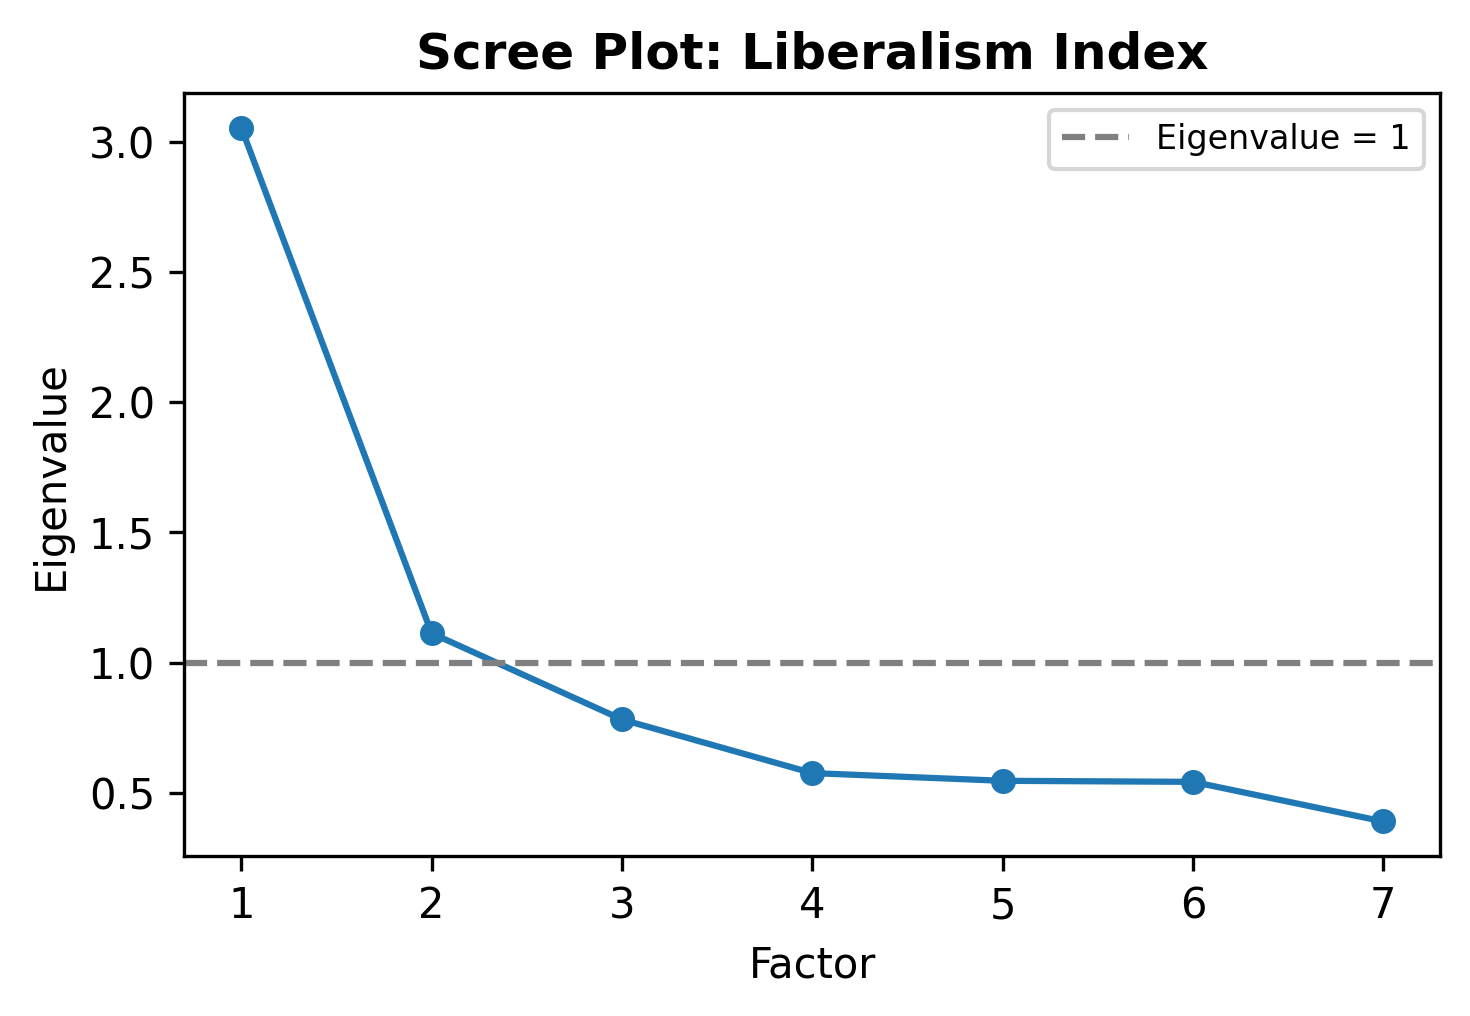
\includegraphics[width=8cm,height=\textheight,keepaspectratio]{images/screeplot_liberal.png}

}

\caption{Scree Plot: Eigenvalues for the Liberalism Index}

\end{figure}%

\subsubsection{Index Rescaling}\label{index-rescaling}

Factor scores on the first factor were extracted and rescaled to the
unit interval {[}0, 1{]} using min--max normalization. Higher values
indicate stronger endorsement of liberal democratic norms. This
transformation does not affect the relative positioning of respondents
on the latent trait. The resulting index has a mean of 0.205 and a
standard deviation of 0.169, with a range from 0 to 1 across 5,324
non-missing respondents.

\subsection{RD Results}\label{rd-results-1}

The coefficient plot below presents all three estimate types
(conventional, bias-corrected, and bias-corrected with robust standard
errors) side by side for each subgroup and model specification.

\begin{figure}[H]

{\centering 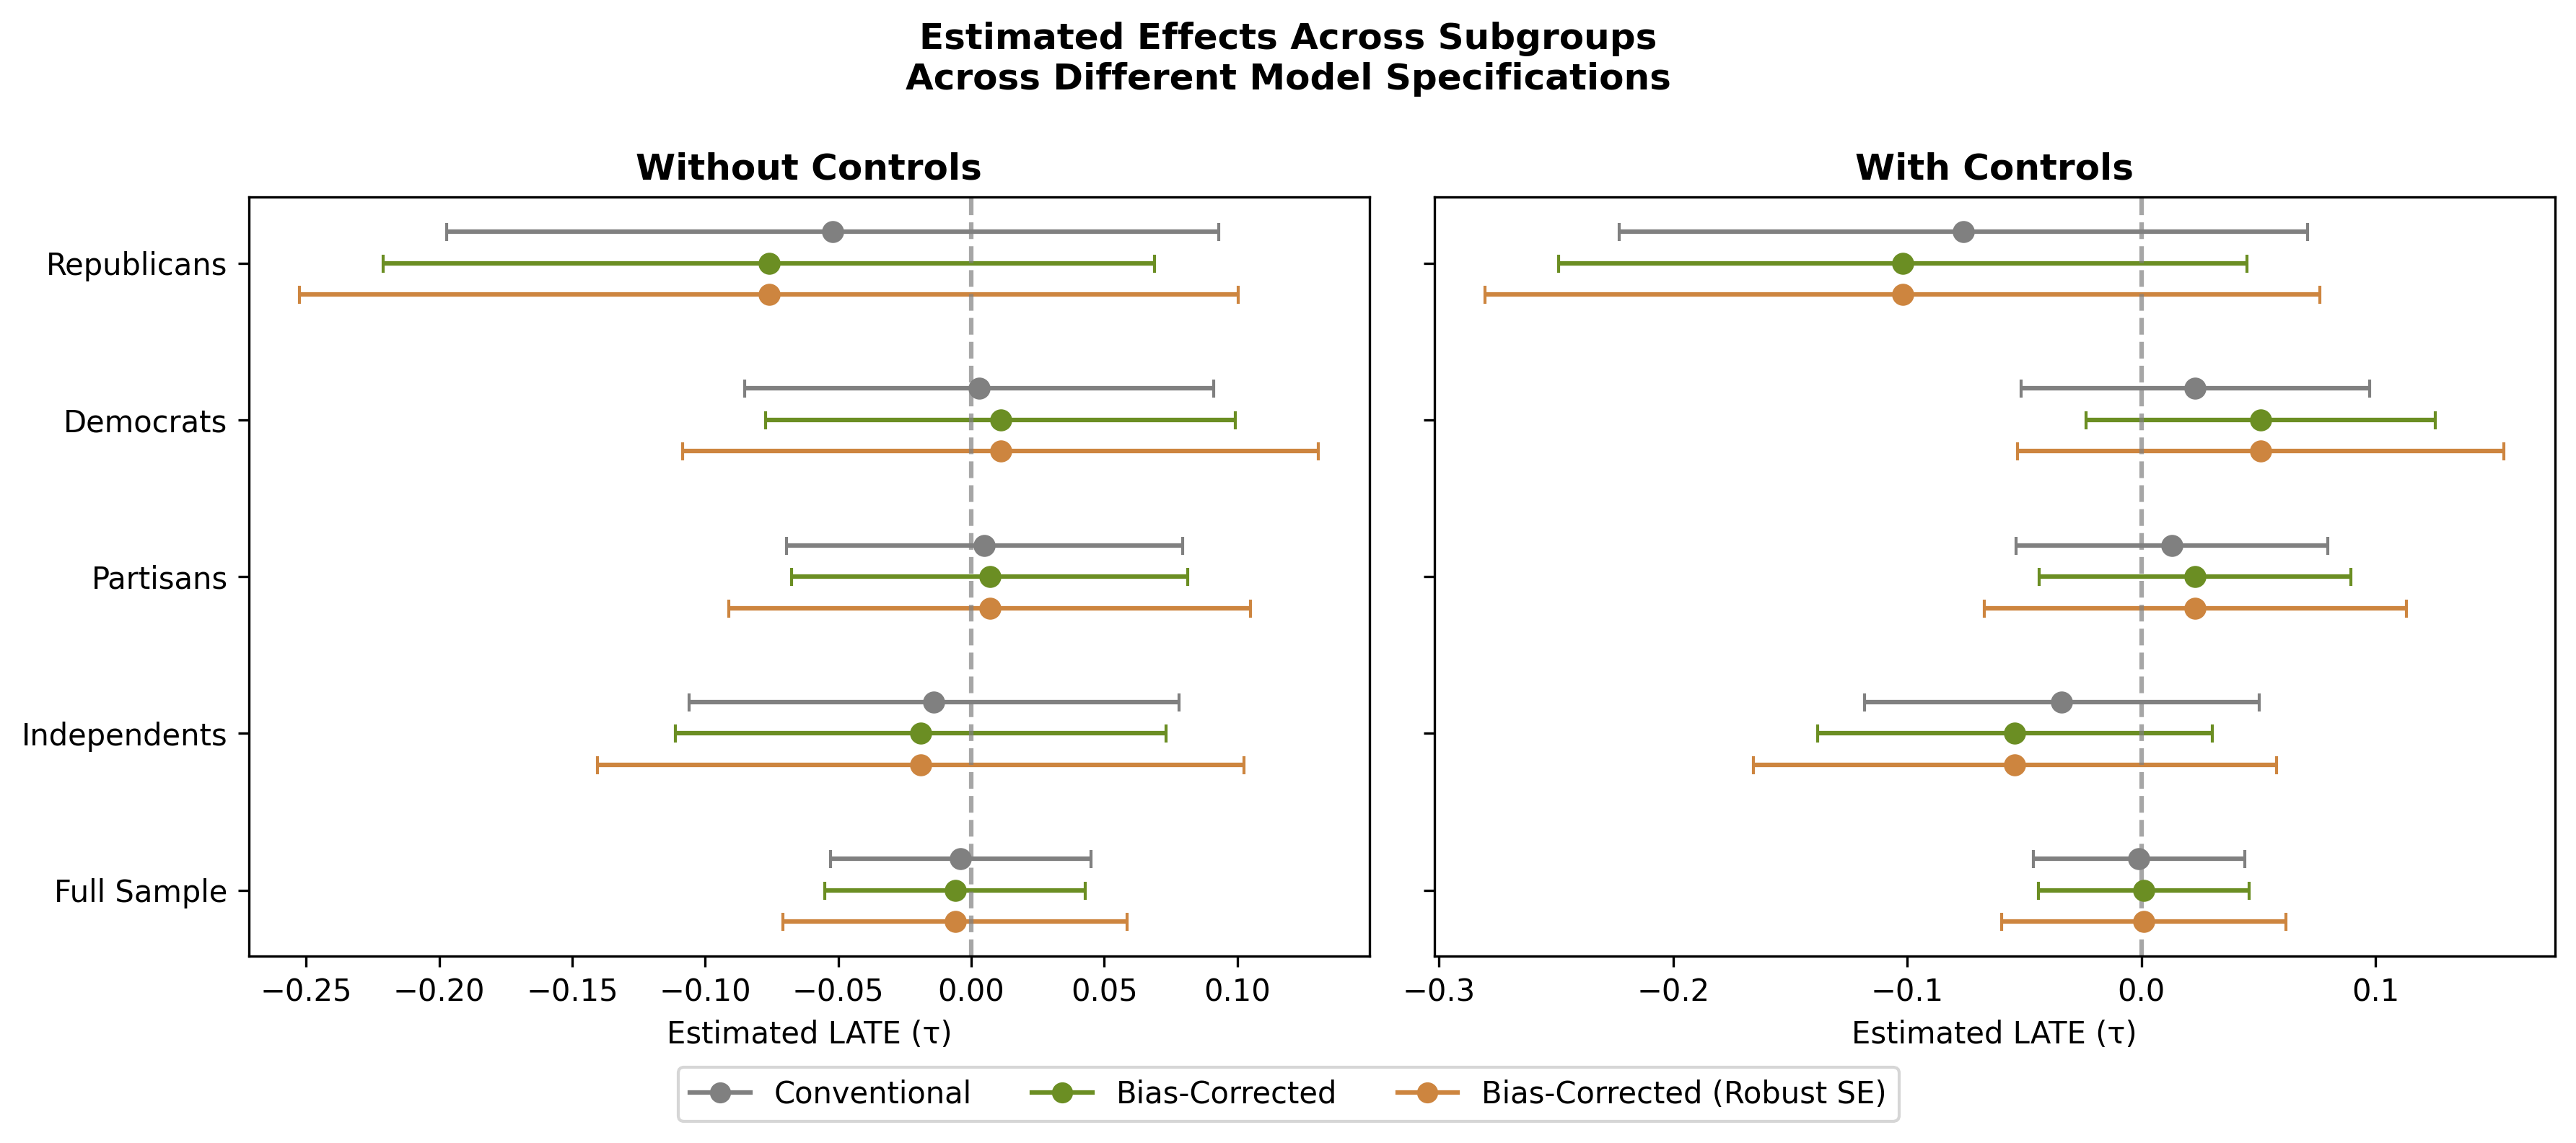
\includegraphics[width=17cm,height=\textheight,keepaspectratio]{images/coefplot_robustness.png}

}

\caption{Comparison of all three RD estimate types (conventional,
bias-corrected, and bias-corrected with robust standard errors) for the
full sample and all partisan subgroups, with and without controls.}

\end{figure}%

\newpage{}

\subsection{Robustness Checks}\label{robustness-checks-1}

The following figures present the full set of robustness checks
(bandwidth sensitivity, placebo cutoffs, and polynomial degree) for each
subgroup. All plots show bias-corrected estimates with controls. With
the exception of some odd `jumps' in statistical significance in very
low bandwidths, and under some placebo cutoffs, the robustness checks
confirm the lack of statistical significance of the previous findings.

\subsubsection{Full Sample}\label{full-sample}

\begin{figure}[H]

{\centering \pandocbounded{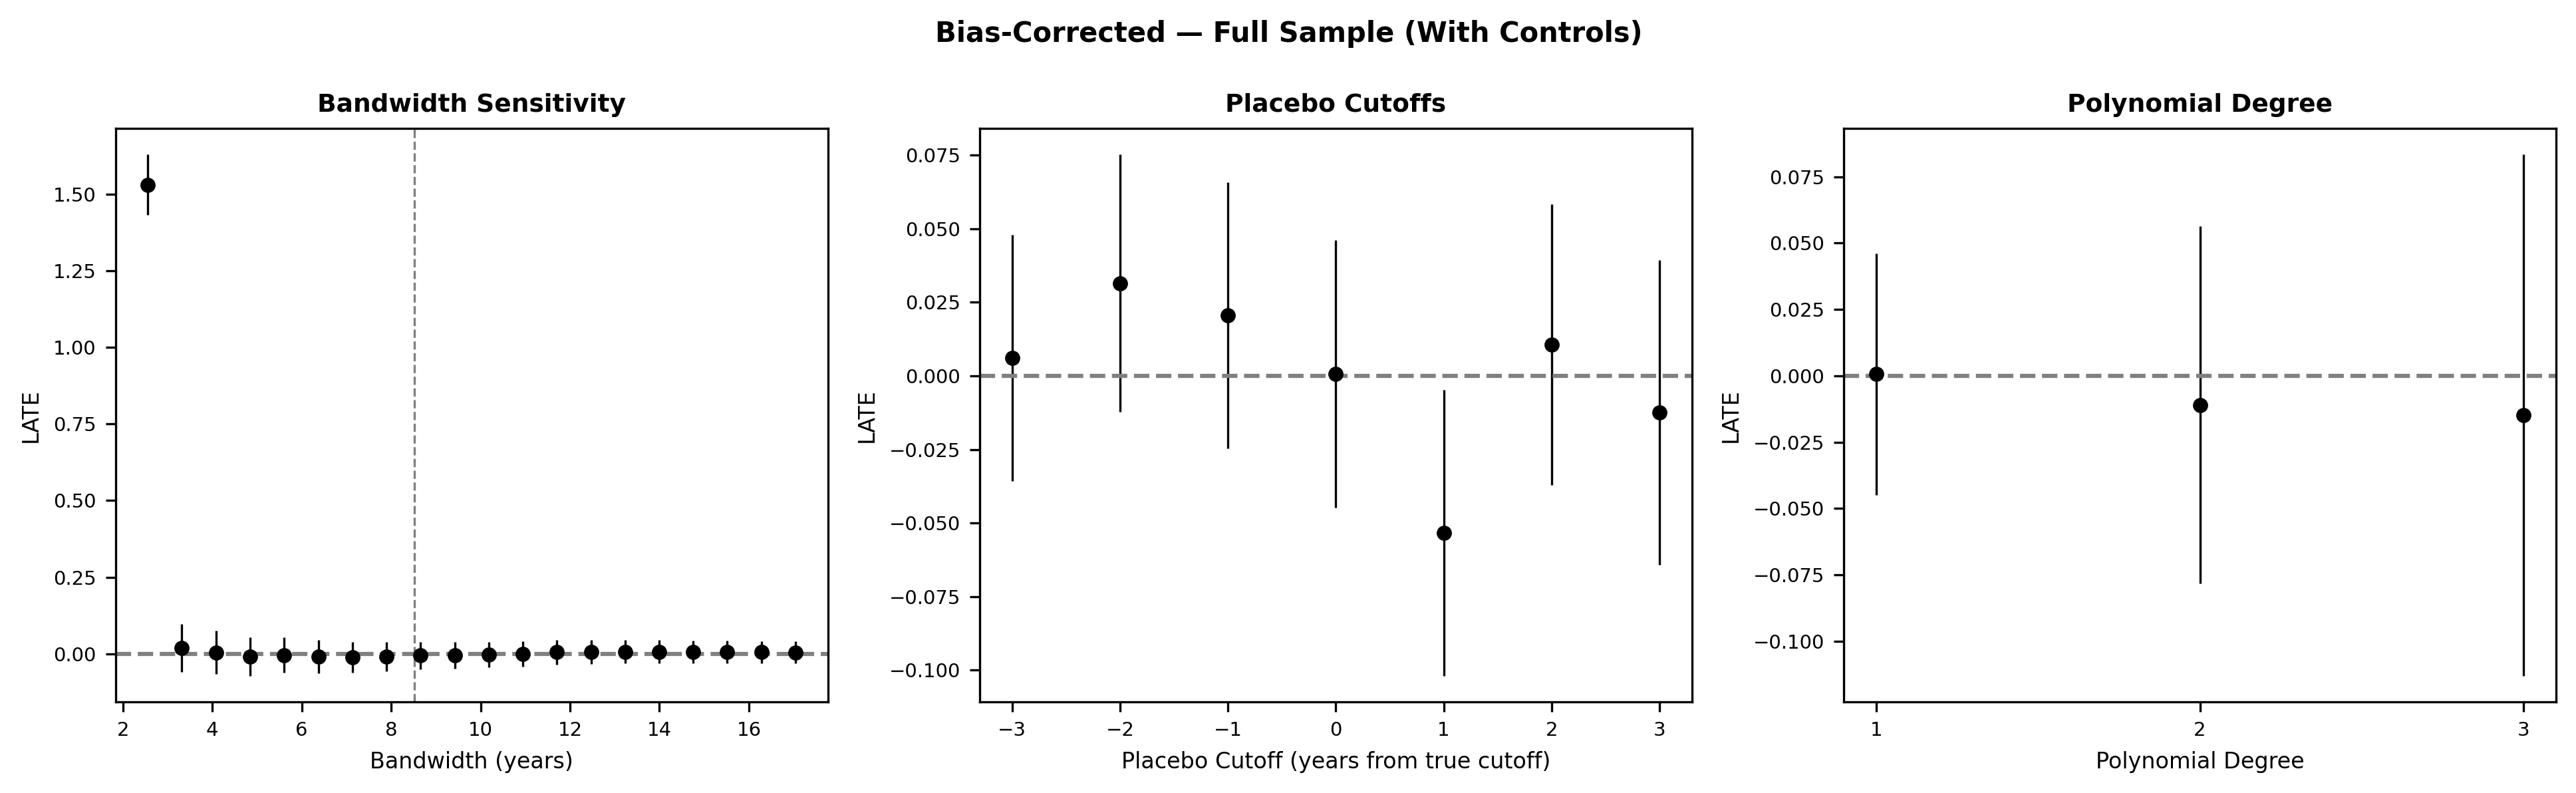
\includegraphics[keepaspectratio]{images/robustness_Full_Sample.png}}

}

\caption{Robustness Checks: Bandwidth Sensitivity, Placebo Cutoffs,
Polynomial Degree (Full Sample)}

\end{figure}%

\subsubsection{Independents}\label{independents}

\begin{figure}[H]

{\centering \pandocbounded{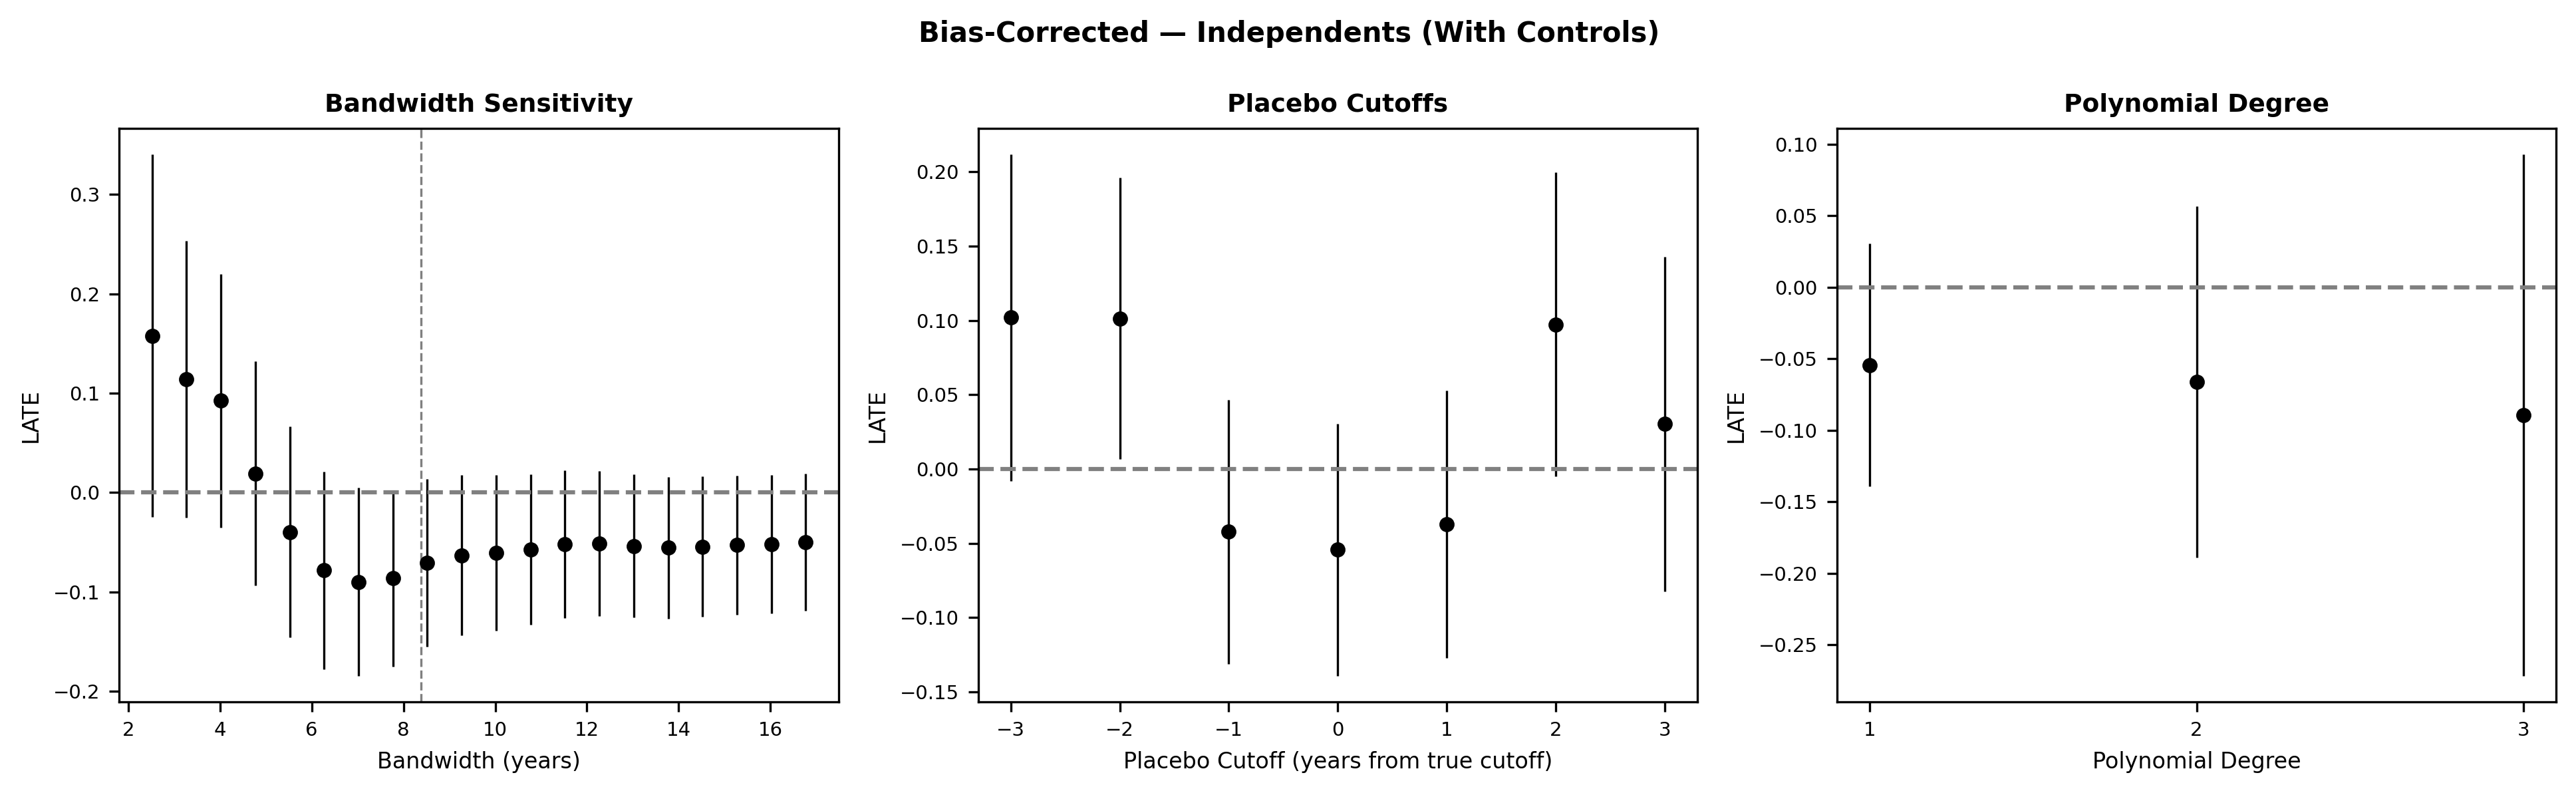
\includegraphics[keepaspectratio]{images/robustness_Independents.png}}

}

\caption{Robustness Checks: Bandwidth Sensitivity, Placebo Cutoffs,
Polynomial Degree (Independents)}

\end{figure}%

\subsubsection{Partisans}\label{partisans}

\begin{figure}[H]

{\centering \pandocbounded{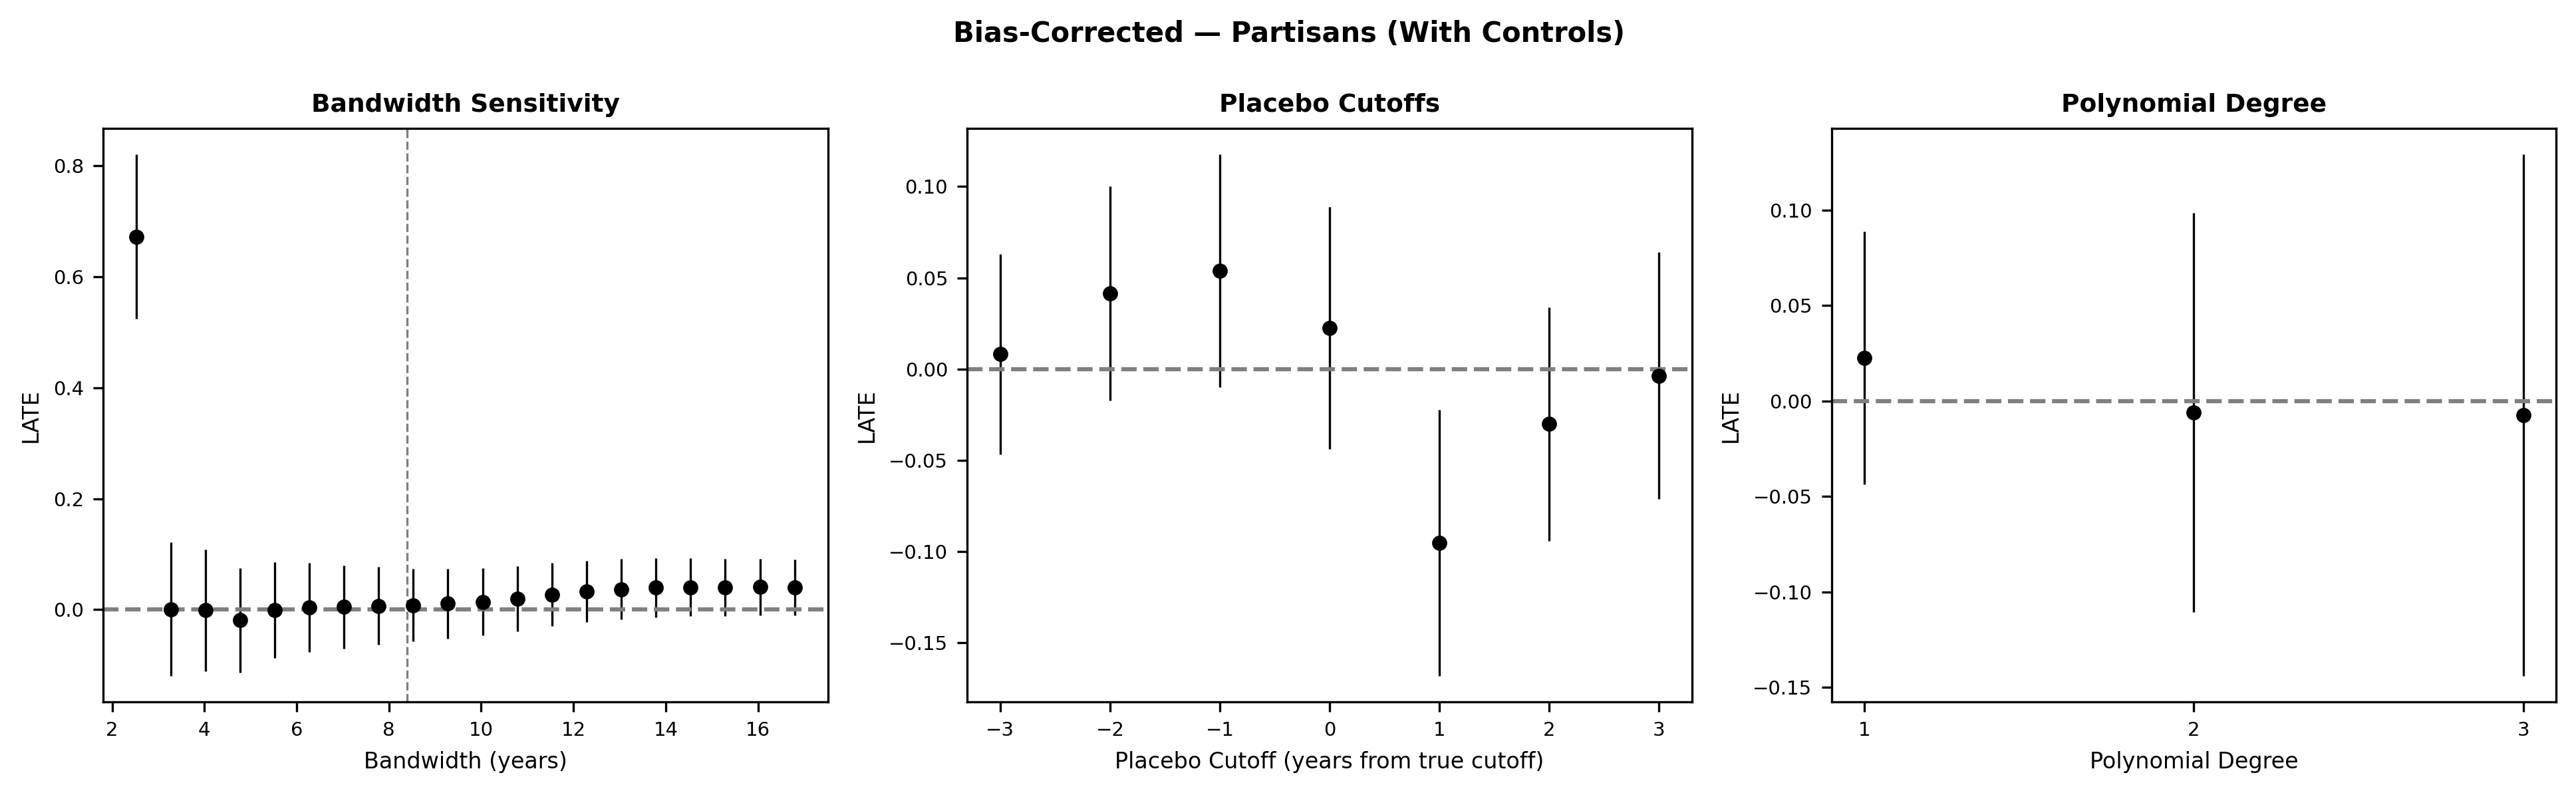
\includegraphics[keepaspectratio]{images/robustness_Partisans.png}}

}

\caption{Robustness Checks: Bandwidth Sensitivity, Placebo Cutoffs,
Polynomial Degree (Partisans)}

\end{figure}%

\subsubsection{Democrats}\label{democrats}

\begin{figure}[H]

{\centering \pandocbounded{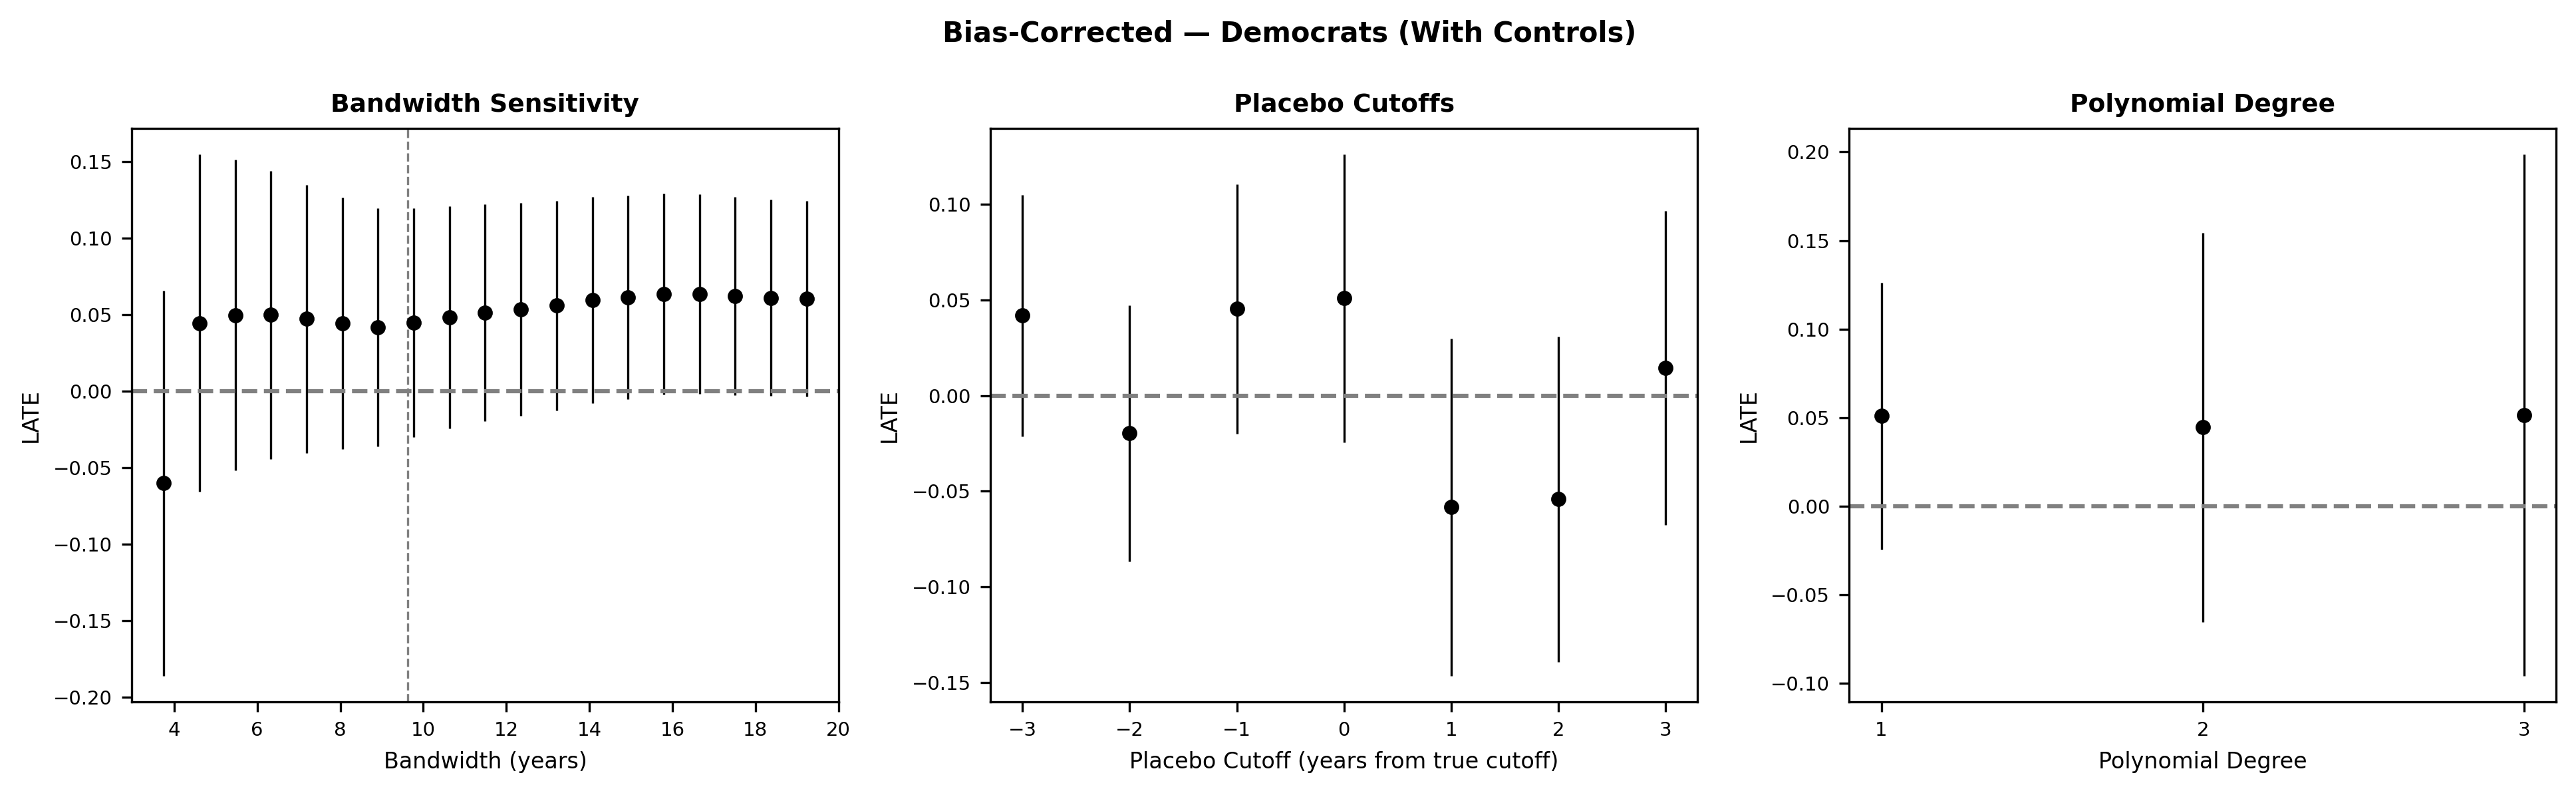
\includegraphics[keepaspectratio]{images/robustness_Democrats-01.png}}

}

\caption{Robustness Checks: Bandwidth Sensitivity, Placebo Cutoffs,
Polynomial Degree (Democrats)}

\end{figure}%

\subsubsection{Republicans}\label{republicans}

\begin{figure}[H]

{\centering \pandocbounded{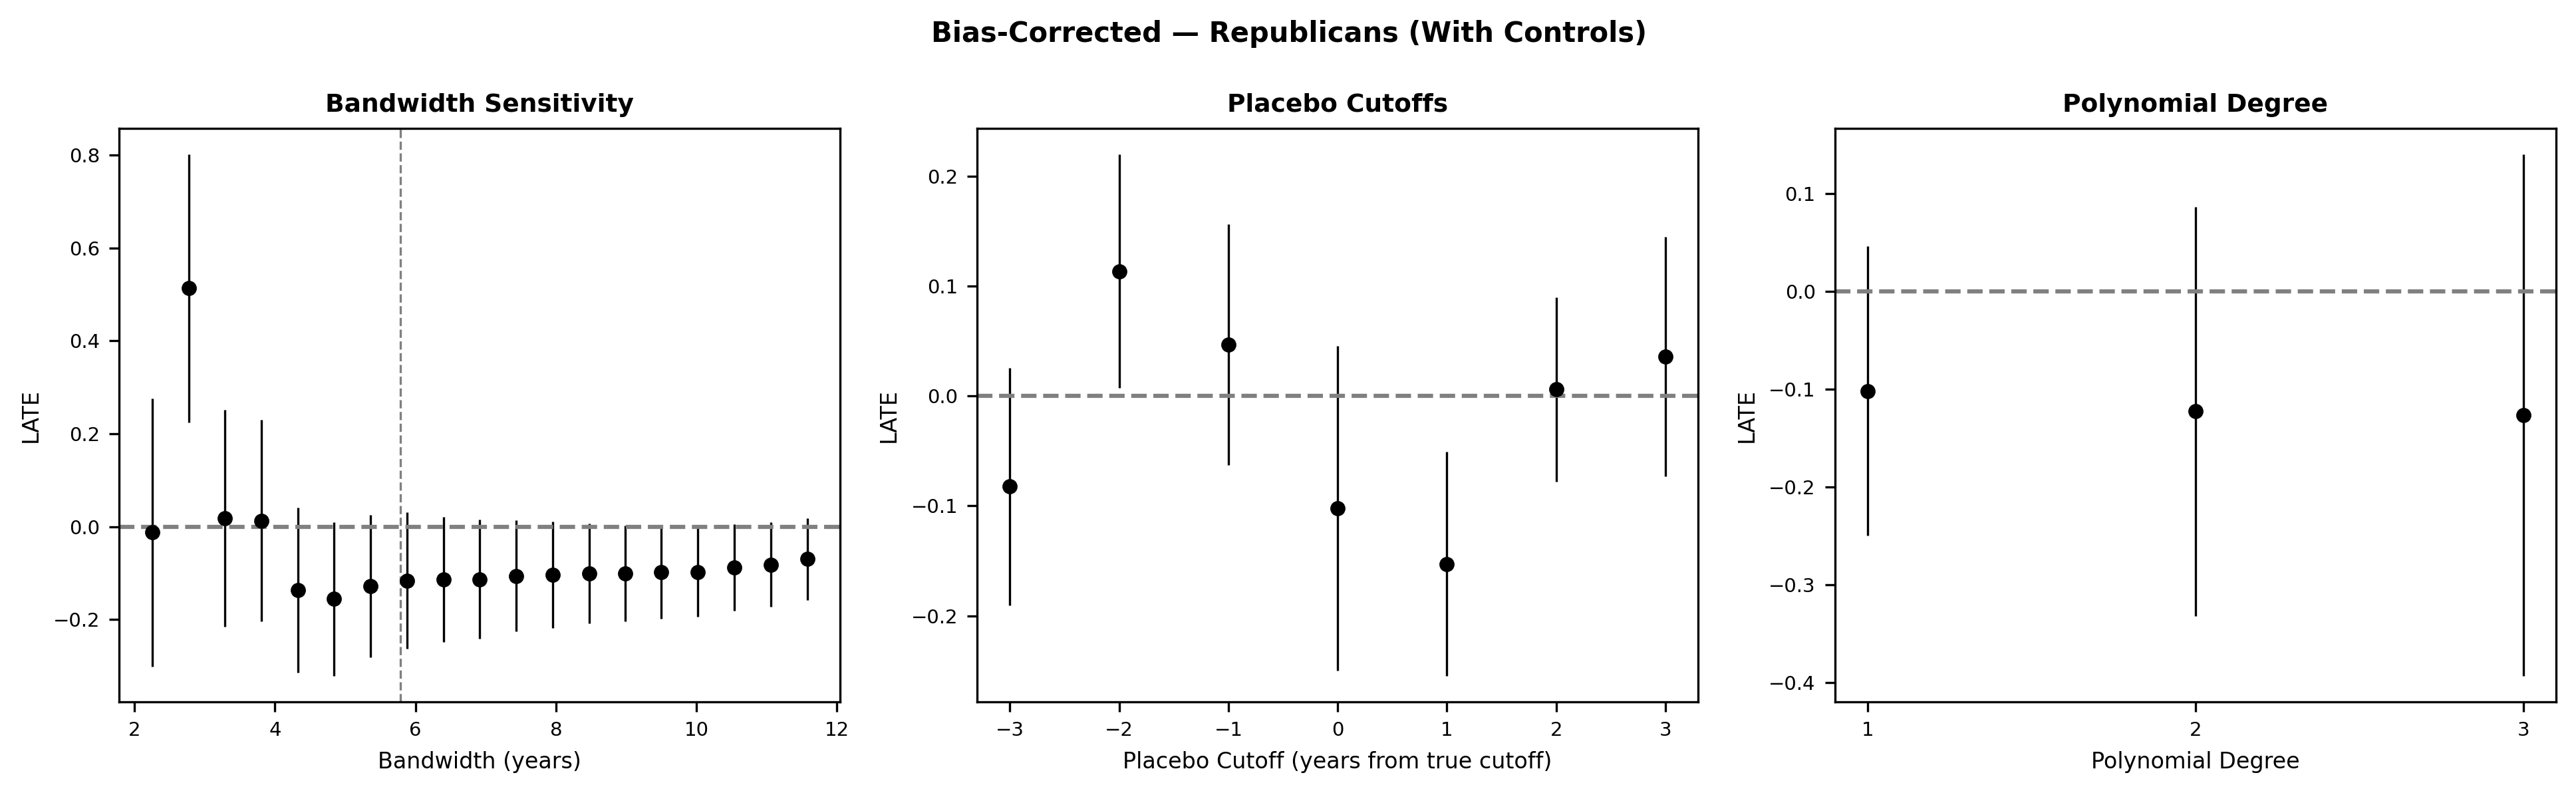
\includegraphics[keepaspectratio]{images/robustness_Republicans-01.png}}

}

\caption{Robustness Checks: Bandwidth Sensitivity, Placebo Cutoffs,
Polynomial Degree (Republicans)}

\end{figure}%




\end{document}
